\documentclass[DM,lsstdraft,toc]{lsstdoc}
\usepackage{graphicx}
\usepackage{url}
\usepackage{color}

\title[LSST Photo-$z$]{LSST DRP (Level 2) \\ Catalog Photometric Redshifts}

\author{M.~L.~Graham}

\setDocRef{DMTN-049}
\date{\today}
\setDocRevision{TBD}
\setDocStatus{draft}

\setDocAbstract{The purpose of this document is to begin to assemble the diversity of motivations driving the inclusion of photometric redshifts in the LSST Level 2 Object Catalog, and prepare to make a decision on what kind of photo-$z$ products will be used. The roadmap for this process is described in Section \ref{sec:intro}. We consider the photo-$z$ use-cases in order to validate that the type of photo-$z$ incorporated into the Level 2 DRP catalog, and the format in which it is stored, meets the needs of both DM and the community. We also compile potential evaluation methods for photo-$z$ algorithms, and demonstrate these options by applying them to the photo-$z$ results of two off-the-shelf photo-$z$ estimators. The long-term plan is for this document to develop over time and eventually describe the decision-making process and the details of the selected algorithm(s) and products. \textbf{Preliminary recommendations can be found in Section \ref{sec:intro}.}}

\setDocChangeRecord{%
\addtohist{1}{2017-04-??}{Initial release of preliminary investigation.}{Melissa Graham}
%\addtohist{2}{yyyy-mm-dd}{Future changes}{Future person}
}

\begin{document}

\maketitle

% CITATION EXAMPLES
% \verb|\citellp|: \citellp{LPM-17, LSE-30} \\
% \verb|\citell|: (SRD; \citell{LPM-17,LSE-29}) \\
% \verb|\citep[][]|: \citep[e.g.,][are interesting]{LPM-17,LSE-29} \\
% \verb|\cite|: \cite{LPM-17,LSE-29}



% % % % % % % % % % % % % % % % % % % % % % % % % % % % % % % % % %
\section{Introduction} \label{sec:intro}

\subsection{Roadmap for LSST Level 2 DRP Photo-$z$}\label{ssec:intro_roadmap}

This roadmap is directly from comments by Mario Juri\'{c} on the Jira thread\footnote{If you have permissions, access at \url{https://jira.lsstcorp.org/browse/DM-6367}}.

The process for the definition of the L2 photo-z data product is the same as for any other data product that isn't fully defined yet. The canonical steps are:
\begin{enumerate}
\item DM Project Science (acting on behalf of overall Project Science) consults with the community (represented by the relevant collaboration -- in this case, the DESC) for options and proposals as to what form of the data product is needed, and the selection of the appropriate algorithm. While it is likely that we will adopt what the DESC recommends, it's likely there will be some iterating to converge to a scientifically acceptable yet implementable solution (e.g. the recommended algorithm may run afoul of our computational, storage, or budget limitations; also DESC may not be the only group concerned about the photo-z product and its properties).
\item Following that (iterative) consultation, DM will recommend (and the Project will select) the Photo-Z algorithm and the data product format, for use in Level 2.
\item DM will implement the selected algorithm. We will, of course, use whatever we can transfer over from DESC (or other) work, but our requirements may be higher than DESC's (e.g., we need to run it reliably in LSST's production environment).
\item DM will implement anything needed to integrate, QC, QA the photo-z data product in data releases (and everything leading up to those; e.g., commissioning). We will, of course, make use of any code and/or help from the DESC, but it is the Project deliverable.
\end{enumerate}

\subsection{Preliminary Recommendations}\label{ssec:intro_pr}

This is a summary of recommendations that were inspired by this work. These recommendations also appear in the relevant sections in the rest of the document. These sections are noted at the end of every item.

\begin{enumerate}
\item DM should write down their plans regarding whether and how the \texttt{Object} database's photo-$z$ will be used in the calibration and/or QA processes, and/or if there will be a separate, internal-use photo-$z$ for this purpose, perhaps in a different database. (Section \ref{ssec:motivation_internal})
\item DM should update the \DPDD to include the fact that each \texttt{Object.Source} will have a link to its own unique version of the normalized system response that includes the filter transmission function ($\phi$, Eq. 5 in the \SRD); this is an important quantity for photo-$z$ and the SC need to know of it's existence and format. (Section \ref{sec:format})
\item Related to above, DM should establish a timeline for developing the algorithm (or releasing this algorithm, if it is already in place) that will be used to standardize the effective filter curves when generating the CoAdds, and verifying how well it meets specifications (e.g., systematics $\sim 0.005$ magnitudes). (Section \ref{sec:format})
\item DM should expand the number of database elements allotted to photo-$z$ from just the \texttt{float[2x100]} that will contain the $P(z)$ by adding one \texttt{float[4]} for a ``best'' photometric redshift and it's uncertainty (mean, median, 68\%, 95\%), and one e.g., \texttt{float[1]}, to encode the best-fit SED template (or synthesized mix of templates) when applicable. However, using 5 of the allocated 200 floats would probably be a suitable compromise. (Section \ref{sec:format})
\item DM should establish a timeline for this process and propose a deadline for the decision regarding the process for generating the photo-$z$ and how they will be stored in the Level 2 database.
\item DM should continue to interact with the Science Collaborations to validate that the specifications related to the Level 2 DRP catalog's photo-$z$ meet their needs. One option may be to officially request the report from the Pitt photo-$z$ meeting which is in preparation and would provide useful input.
\end{enumerate}


% % % % % % % % % % % % % % % % % % % % % % % % % % % % % % % % % %
\section{Use-Cases as Motivation for the Level 2 Photo-$z$ Estimator(s)}\label{sec:motivation}

In this section we describe the internal and external motivations for why photo-$z$ are being included in the Level 2 database and how they influence our choice of photo-$z$ algorithm. Typically, photometric redshift algorithms work by either fitting template spectra to the observed photometry or by matching photometry to a training set of galaxies with spectroscopic redshifts. The method of ``matching photometry'' is often done with machine learning codes. Hybrid photo-$z$ estimators also exist, attempting to mitigate the flaws of either process (e.g., the SDSS DR12 photo-$z$ estimator by \citealt{2016MNRAS.460.1371B}, or the Gaussian Processes estimator described by \citealt{2017ApJ...838....5L}). To know which kind of photo-$z$ estimator(s) LSST will need, we start by collecting the various motivations for including a photo-$z$ estimate in the Level 2 catalogs.

\subsection{Internal Requirements}\label{ssec:motivation_internal}

The relevant requirement is DMS-REQ-0046 (see \citeds{LSE-61}), ``The DMS shall compute a photometric redshift for all detected Objects.'' From the Jira conversation\footnote{If you have permissions, access at \url{https://jira.lsstcorp.org/browse/DM-6367}} on this issue we've managed to cobble together some potential internal uses for a Level 2 photo-$z$, and list them below (leaving the quotes unattributed). Although they are vague, all of these seem to suggest at least implicitly that a template-fitting code would be used to generate the photo-$z$:
\begin{itemize}
\item {\it ``DM would like to be able to run some sort of photo-z code for QA purposes ... good enough to validate LSST's galaxy photometry''}. Using observed SED of real galaxies seems like the best choice for validating photometry, e.g., if the question is whether the photometric outputs match the colors of real galaxies.
\item DM {\it ``should definitely also run some sort of photometric cluster finder for QA purposes, which provides much better photo-zs for red cluster galaxies and hence gives us much better photometric quality tests for a small subset of the population ... idea is that the width of the red sequence in clusters is really the only simple metric we have for galaxy photometry colors that doesn't rely on simulations''}. However, photo-$z$ might not actually be involved in this metric, as the code uses ``the colors of the galaxies directly to estimate the red sequence, rather than relying on photo-zs (which have a lot of assumptions built in already).'' If photo-$z$ for red sequence galaxies are being prioritized, perhaps the best results would be generated by fitting elliptical galaxy spectra only. Also, we'd need to test whether template-fitting or machine-learning is best for that particular scenario.
\item {\it ``DM is already on the hook for some sort of photo-z in the form of SED fitting (and I would assume templates/redshifts) for chromatic corrections''}. In this case, it sounds like SED fitting is the only option that would satisfy the use case of chromatic corrections.
\end{itemize}

Reconciling the photo-$z$ option that best suits internal needs with external might be quite difficult and furthermore, unnecessary. Jeff Newman from DESC-PZ commented that the internal-use photo-$z$ \textit{``will almost certainly be different/simpler photo-$z$s than the database ones.''}

\textbf{Recommendation: DM should write down their plans regarding whether and how the \texttt{Object} database's photo-$z$ will be used in the calibration and/or QA processes, and/or if there will be a separate, internal-use photo-$z$ for this purpose, perhaps in a different databse.}

\subsection{External Requirements}\label{ssec:motivation_external}

Extragalactic astrophysics such as weak lensing, baryon acoustic oscillations, and Type Ia supernova cosmology are all main science drivers for the LSST, and all require catalogs of galaxies with photometric redshifts. However, the photo-$z$ algorithms for precision cosmology will be custom-tailored to the needs of each domain and we should consider those applications as Level 3 photometric redshifts. Instead, the main consumers of the Level 2 photo-$z$ product will probably be users wanting to do things like:
\begin{itemize}
\item evaluate the cluster membership status of galaxies (e.g., for spectroscopic follow-up campaigns)
\item reject compact extragalactic objects from stellar samples, or vice versa (e.g., for spectroscopic follow-up campaigns)
\item identify and/or characterize extragalactic transient host galaxies (sometimes the transient redshift is known and used to identify the host, and sometimes the most probable host is used to constrain the transient redshift)
\item begin their cosmological studies as soon as possible, before the Level 3 photometric redshift routines are perfected
\item additionally some advanced/specialized science may start with the Level 2 photo-$z$ and then apply calibrations, adjustments, or cuts on top of that in order to use them (e.g., maybe weak lensing studies; from a conversation with H. Hildebrandt)
\end{itemize}

\smallskip
The chosen Level 2 photo-$z$ algorithm(s) should be easily understandable and characterizable, and the output photometric redshifts and their uncertainties should be strictly defined. If a tradeoff needs to be made, it will probably be more important for the uncertainties to be reliable than for the photo-$z$ to be more accurate (to a point, of course). To maximize early science capabilities of the scientific community we should consider algorithms that will return the most accurate photo-$z$ as early in the survey as possible. For this reason, in Section \ref{sec:options} we begin to set up a framework for a performance analysis of photo-$z$ from galaxy catalogs simulated to resemble LSST data at 1, 2, 5 and 10 years.

\smallskip
In the future we will be be in touch with the extragalactic LSST Science Collaborations for input (and we are already in touch with the DESC photo-$z$ WG). We will do this by contacting the chairs of following SC: Galaxies, Dark Energy, Active Galactic Nuclei, Transients, and Strong Lensing (unless the latter has become the DESC SL WG). We may also want to include the Stars, Milky Way, and Local Volume SC, to see if they rely on photo-$z$ to reject objects from their sample. One option would be to identify a point of contact that we can converse with, or another option would be to poll the general community. If we want to do a poll, perhaps questions like this would be useful.
\begin{enumerate}
\item Please rate how important LSST-provided photometric redshifts are to your science goals, e.g., on a scale of 1 to 5 (not important, insignificant, useful, important, essential).
\item Please rate how well the proposed LSST-provided photo-$z$ meet your science needs, e.g., on a scale from 1 to 5 (not met, poorly met, adequate, well met, perfectly met).
\item Regardless of your answer to 2, please rate how often you might use the proposed LSST-provided photometric redshifts, e.g., on a scale of 1 to 5 (never, rarely, occasionally, regularly, always).
\end{enumerate}

\subsection{Requirements Summary}

The initial impression is that DM/QA might require a template-fitting estimator, and that machine-learning codes would be less favorable because they require a deep training set be made in advance (i.e., from the 10-year equivalent commissioning field).


% % % % % % % % % % % % % % % % % % % % % % % % % % % % % % % % % %
\section{Format of Photo-$z$ in Level 2 Catalog}\label{sec:format}

In this Section we discuss the format of the photo-$z$ in the Level 2 catalog and options for compression. The photometric redshift products that the LSST DM team will provide in the Level 2 object catalogs are defined in \DPDD, Table 4, ``Level 2 Catalog Object Table'' as:
\begin{itemize}
\item \texttt{stdColor} = ``standard color'', color of the object measured in ``standard seeing,'' suitable for photo-z
\item \texttt{stdColorErr} = uncertainty on stdColor
\item \texttt{photoZ (float[2x100])} = photometric redshift likelihood samples, pairs of redshift and likelihood ($z,\log{L}$), computed using a published and widely accepted algorithm at the time of LSST
\end{itemize}

\noindent This desired format is set for an algorithm that returns $z,logL$, as opposed to a single ``best'' value and error, but as most estimators do return a posterior probability density function this is not a restrictive constraint. The posterior PDF will need to be compressed for storage within a \texttt{float[2x100]} array.

There are additional quantities that will be useful for Level 3 photo-$z$. The DESC photo-$z$ WG has suggested that the DM-provided Level 2 DRP photo-z should be one that incorporates effective filter transmission curves for each individual epoch, because the required processing power for this is likely beyond the scope of any Level 3 photo-z estimator. However, \v{Z}eljko responded on the Jira thread that:

\begin{quote}
{\it ``Although the Source table in \DPDD doesn't list it explicitly (calibration docs do, but they are in state of flux right now), each Source must know (have a link to) its own transmission function (phi, see eq. 5 in the \SRD). Once you know phi, and its standard version, phi\_std, and you assume an SED, it's straightforward to compute photometric offset between the phi and phi\_std systems. In practice, it will be somewhat more involved because we have a probabilistic photo-z, which implies a probabilistic, and not deterministic, SED.''}
\end{quote}

\textbf{Recommendation:  DM should update the \DPDD to include the fact that each \texttt{Object.Source} will have a link to its own unique version of the normalized system response that includes the filter transmission function ($\phi$, Eq. 5 in the SRD); this is an important quantity for photo-$z$ and the SC will want to know of it's existence and format.}

\textbf{Recommendation: DM should establish a timeline for developing the algorithm (or releasing this algorithm, if it is already in place) that will be used to standardize the effective filter curves when generating the CoAdds, and verifying how well it meets specifications (e.g., systematics $\sim 0.005$ magnitudes).}

\subsection{Compression}\label{ssec:format_compression}

Efficient $P(z)$ compression algorithms are in development. \cite{2014MNRAS.441.3550C} present an alternative method for storing photo-$z$ PDFs that requires less storage space. With their algorithm for sparse representation, ``an entire PDF can be stored by using a 4-byte integer per basis function.'' As they describe, ``only ten to twenty points per galaxy are sufficient to reconstruct both the individual PDFs and the ensemble redshift distribution, $N(z)$, to an accuracy of 99.9\% when compared to the one built using the original PDFs computed with a resolution of $\delta z = 0.01$, reducing the required storage of two hundred original values by a factor of ten to twenty.'' The advantage in this method seems to be the accuracy, and the disadvantage is that the science user would need to convert the stored format into a $P(z)$ before they can use it (minor drawback). It is unclear to me how much additional processing is required for this conversion, and whether this is within DM's computational budget. The DESC photo-$z$ WG has indicated that they expect compression techniques to be sufficient to store multiple algorithms' $P(z)$ results into the single database element of \texttt{Object.photoZ (float[2x100])}. This will increase both the advantages of compression and the required processing time. Also, Phil Marshall and Alex Malz are currently working on photo-$z$ compression (2017-04-12).
%From our analysis in Section \ref{sec:options}, we look at the output from the BPZ code with a galaxy catalog simulated for a 1 year LSST survey to get an idea of the amount of information in a PDF. Approximately 50\% of all test galaxies had a $P(z)$ with $>100$ elements with $P>0.000$ when a resolution of $\delta z = 0.01$ was used. This fraction drops to 6\% of galaxies with $>100$ elements with $P>0.005$. This suggests it might be possible to do a really simple compression down to 100 elements by, e.g., combining adjacent low-probability bins in some efficient fashion until the number of bins is $=100$. No bins with $>1\%$ of the probability would need to be combined, and while some information would be lost, the benefit for the science user is that the posterior PDF is a simple machine-readable ascii table. However, in practice, many more complicated and

\subsection{Proposed Alterations}\label{ssec:format_summary}

Two low-priority suggestions for minor changes to the photo-$z$ content in the Level 2 database. (1) Many science users will simply want the photo-$z$ and its uncertainty (e.g., the peak of the PDF and its 68\% confidence interval). We recommend including this separately from the $P(z)$. This could be a separate element in the database or e.g., the first element of \texttt{photoZ}. As these values are natural outcomes of most algorithms they should not increase DM processing. (2) If a template-fitting estimator is used, we need add a database element to store information about the best fit template. We will also have to make the templates publicly available. This information is important because it could help the user to evaluate whether the photo-$z$ is sensible; e.g., allow them to weed out instances when an elliptical SED is best fit to a morphologically spiral object, or similar scenarios.

\textbf{Recommendation: DM should expand the number of database elements allotted to photo-$z$ from just the \texttt{float[2x100]} that will contain the $P(z)$ by adding one \texttt{float[4]} for a ``best'' photometric redshift and it's uncertainty (mean, median, 68\%, 95\%), and one e.g., \texttt{float[1]}, to encode the best-fit SED template (or synthesized mix of templates) when applicable. However, using 5 of the allocated 200 floats would probably be a suitable compromise.}
%Having 100 redshift bins (maximum) for the PDF means that no bin has $<1\%$ of the probability, which is a nice, round number and easy to understand. Although not exactly a science-driven need, perhaps we could simply increase the storage space allotted to \textsc{photoZ} to \textsc{float[2x101]} to accommodate the first elements being used to store the photo-$z$ and error.



% % % % % % % % % % % % % % % % % % % % % % % % % % % % % % % % % %
\section{Potential Options for Photo-$z$ Evaluation}\label{sec:options}

As an extremely preliminary demonstration of the types of tests a given photo-$z$ estimator might undergo during the selection process to determine which will be included in the Level 2 database, we examine the performance of two off-the-shelf photo-$z$ codes. We consider, for now, one template-fitting and one machine-learning estimator. In Section \ref{ssec:options_lit} we cover some existing work that was consulted in compiling these evaluation options. In Section \ref{ssec:cats} we describe the galaxy catalogs that we use. In Section \ref{ssec:estimators} we describe the template-fitting photo-$z$ estimator BPZ and the machine-learning code TPZ. Section \ref{ssec:comp} demonstrates some analysis techniques for comparison of different estimators' photo-$z$ results. We emphasize that the parameters of the estimators themselves have not been optimized to return the most accurate photo-$z$, and some minor mistakes have been made in these initial runs, but that this is fine as we are simply demonstrating an evaluation process. In Section \ref{ssec:more} we write down some ideas for future tests of the photo-$z$ estimators that would evaluate their performance in real world situations, and that are similar to the types of early science that might be done with LSST photo-$z$.


\subsection{Relevant Existing Work}\label{ssec:options_lit}

\textbf{DESC photo-$z$ WG --} This science community is full engaged in the development of photo-$z$ routines and their optimization for LSST. Here we list just other relevant existing work.

\textbf{Relevant photo-$z$ testing papers --} \cite{2010A&A...523A..31H} tested 18 different photo-$z$ codes on the same sets of simulated and real data and found no significantly outstanding method. \cite{2013ApJ...775...93D} test 11 different photo-$z$ codes on the CANDLES data set ($U$-band through infrared) and also find that no method stands out as the ``best,'' and that there is a strong dependence of photo-$z$ accuracy on the SNR of the photometry (relevant for our tests at 1 year). They also found that most of the photo-$z$ codes underestimate their redshift errors, which is important to note because we do want accurate errors.

\textbf{Lessons from DES --} \cite{2014MNRAS.445.1482S} use the science verification data (200 square degrees of $grizY$ photometry to a depth of $i_{AB}=24$ magnitudes) of the Dark Energy Survey (DES) to evaluate several photometric redshift estimators. They found that the Trees for Photo-z code (TPZ; \citealt{2013ascl.soft04011C}) provided the most accurate results with the highest redshift resolution, and that template-fitting methods also performed well -- especially with priors -- but that in general there was no clear ``winner.''

\textbf{Lessons from SDSS --} \cite{2016MNRAS.460.1371B} describes the photo-$z$ adopted for the SDSS DR12. As I understand it, they first use an empirical technique with a large training set to estimate the redshift and it's error, and then fit SED templates with that redshift in order to obtain additional galaxy information such as $K$-correction and spectral type. (Note: \textit{They call it a hybrid technique but the photo-$z$ sounds like it comes solely from the local linear regression, basically an interpolation in the color-redshift relation}.)

\textbf{Lessons from Lucy's work --} Lucy Halperin used what we call ``Brown'' catalog\footnote{We call it the Brown catalog because it uses the SEDs from \cite{2014ApJS..212...18B}} made by Sam Schmidt with simulated 10-year LSST-like magnitude uncertainties and ran it through 2 machine learning (ANNz and TPZ) and 2 template-fitting (LePhare and BPZ) photo-$z$ codes. All four returned sets of photo-$z$ with similar standard deviations and biases, but the template-fitting codes were more prone to failures and outliers. We found that for template-fitting photo-$z$ codes, the choice of template SED set does make a significant difference in the results, particularly regarding photo-$z$ outliers -- however, this may have been particular to our use of the ``Brown''-based galaxy catalog. We do not use this catalog in Section \ref{sec:options}.

\subsection{Simulated Catalogs}\label{ssec:cats}

We use a randomly chosen 30000 galaxy test subset of the \textsc{LC\_DEEP\_Gonzalez2014a} catalog, which is based on the Millennium simulation \citep{2005Natur.435..629S} and the galaxy formation models of \cite{2014MNRAS.439..264G} and constructed using the lightcone techniques described by \cite{2013MNRAS.429..556M}. We impose a limit on the true catalog redshift of $z<3.5$, and a limit on the apparent $i$-band magnitude of $i<25.5$, and furthermore require galaxies to be detected in the three filters $gri$. The latter requirement means that the test galaxies' apparent magnitude is brighter than a limit defined by a signal-to-noise ratio $<5$ in all three filters $gri$. This limit depends on the number of years of survey elapsed, and since we want to use the same set of test galaxies to analyze the algorithms' results early in the survey, we require this $gri$ non-detection with the expected limits after only 1 year of LSST. These restrictions mean that we end up with a catalog that has with fewer faint galaxies than will be in the LSST 10-year catalogs, and so the 10-year results we consider here are optimistic (but that's fine for our purposes). These restrictions are imposed prior to the random selection of 30000 test galaxies from the larger catalog. We then simulate 4 versions of the test galaxy catalog with errors appropriate for $1$, $2$, $5$, and $10$ years of LSST. We calculate galaxy magnitude uncertainties that are appropriate for the elapsed survey time, and observed photometry is simulated by adding a random scatter proportional to the uncertainties.

In addition to the test set, we need a training set of galaxies for the machine-learning algorithm to serve as a spectroscopic redshift catalog. Spectroscopic data sets containing tens of thousands of galaxies down to $i>25$ and out to $z>3$ are certainly possible, e.g., the VIMOS Ultra Deep Survey (VUDS; \citealt{2015A&A...576A..79L}). Assuming that the LSST will cover a spectroscopic field like the VUDS to the full 10-year depth during commissioning or with a first-year deep drilling field, we use as our training set a sample of 30000 catalog galaxies with photometric uncertainties equivalent to a 10-year LSST. This training set has the same redshift and magnitude distribution and limits as the galaxy catalogs, which may not be the case for a real spectroscopic set.

\subsection{Example Photo-$z$ Estimators}\label{ssec:estimators}

\textbf{Bayesian Photometric Redshifts} (BPZ; \citealt{2000ApJ...536..571B}) is a template-fitting algorithm with a magnitude prior\footnote{\url{http://www.stsci.edu/~dcoe/BPZ/}}. We use all default parameters, including the $i$-band for the magnitude prior, except that we supply the CFHTLS set of SED templates. This set is 66 SEDs that were used for the CFHTLS photo-z paper and are from \cite{2006A&A...457..841I}, and they were interpolated from the CWW and Kinney models.

%Note: run with 100 trees was 1h 47m.
\textbf{Trees for Photometric Redshifts} (TPZ; \citealt{2013ascl.soft04011C,2013MNRAS.432.1483C}) is a machine learning algorithm that uses prediction trees and a training set of galaxies with known redshifts. We use all the default parameters from the example, except we increase the number of trees from 4 to 10 (this was set low in the provided example to decrease run time). Since the number of realizations is 2, this is a total of 20 trees. As shown in \cite{2013MNRAS.432.1483C}, the bias and scatter of the resulting photo-$z$ improve the most as the number of trees is increased to 20, and continues to improve more mildly to 100, and then are not much improved beyond 100 trees (i.e., their Figure 9). We also set the maximum redshift to 3.5 and the number of redshift bins to 350. We include both magnitudes and colors and their uncertainties as attributes to be used in the prediction trees, as Lucy's work found that this led to better results. From the TPZ output files, we take as $z_\mathrm{phot}$ the mode of the redshift distribution instead of the mean because this is the peak of the distribution (most likely redshift). \textit{Note: I may have misunderstood how TPZ uses the photometric uncertainties. I thought it treated errors differently from other \texttt{Attributes}, but perhaps it uses them just the same. That makes sense, but means it is inappropriate to include photometric errors as {ttc Attributes} if the train and test sets have different photometric precision.} In case a training set with LSST photometric uncertainties at the level of a 10-year survey is not available from commissioning or a dedicated deep drilling survey by the end of year 1, we also simulate the photo-$z$ results with a training set that has the same level of photometric uncertainty as the test set.

\textbf{Nearest-Neighbors in Color} (NNC; Graham et al. in prep) is a photo-$z$ estimator that uses the Mahalanobis distance in color-space to match a galaxy to a training set. We simulate photo-$z$ at 1, 2, 5, and 10 years using a test set of 20000 and a training set of 60000. Training set has the same photometric depth as the test set.


\subsection{Techniques for Analysis and Comparison of Photo-z Estimators}\label{ssec:comp}

In this section we demonstrate several analysis techniques for comparing the output of different photo-$z$ estimators, discussing each in turn below and then listing some potential future techniques in Section \ref{ssec:more}.

\smallskip \noindent \textbf{The $z_\mathrm{true}$--$z_\mathrm{phot}$ Diagram} \\
Figure \ref{fig:tzpz} shows the photo-$z$ results in $z_\mathrm{true}$--$z_\mathrm{phot}$ diagrams, which are a typical way to visually asses the output. Galaxies are plotted with a semi-transparent black dot so that density and clustering of points is clear, and galaxies that end up designated as ``outliers'' are over-plotted with a more opaque red dot. Problems such as outlier structure from e.g., color-$z$ degeneracies, and quantization of $z_\mathrm{phot}$ is obvious in these kinds of diagrams, as well as a decent overall impression of the scatter and bias. Even though our runs with these estimators have not been optimized, we can make an ``example'' assessment of these figures to compare the two estimators.
\textbf{BPZ:} Overall the results are quite poor even with the LSST 10-year predicted photometry, especially the amount of quantization at $z_\mathrm{phot}>1.5$. We find that the results are not improved if we remove the magnitude prior, or use a different SED template set such as those from \cite{2014ApJS..212...18B}. We do know from Lucy's work that the choice of SED template set has a significant impact on the results (this is actually widely known) -- in Lucy's work, the best results were achieved when we used the Brown SEDs with a galaxy catalog for which the photometry was simulated using those same SEDs. However, it's less straightforward to identify the ``best'' template SEDs to use with the Euclid galaxy catalog (or real data for that matter). \cite{2014MNRAS.439..264G} describes the wide variety of stellar population spectral synthesis models they used, but it would take quite some work to get them all together into a single catalog to provide to BPZ.
\textbf{TPZ:} The results are quite poor 1 and 2 years, with a lot of quantization in the photo-$z$ and many outliers at low and high redshift, but are significantly improved at 10 years. It is very interesting that there is actually a large improvement if the training set does not have better photometric errors than the test set (i.e., compare the 1 and 2 year results in the third row to the second row), but this may just be related to how we've included the errors as \texttt{Attributes}. Either way, TPZ is sensitive to the provided training set, so an extended investigation into what would truly be a realistic 1 year spectroscopic training set for LSST should be done (e.g., different redshift distributions, different magnitude limits). Although TPZ appears to give better accuracy, we also need to ensure that it gives realistic precision for it's photo-$z$ results.

\begin{figure*}
\begin{center}
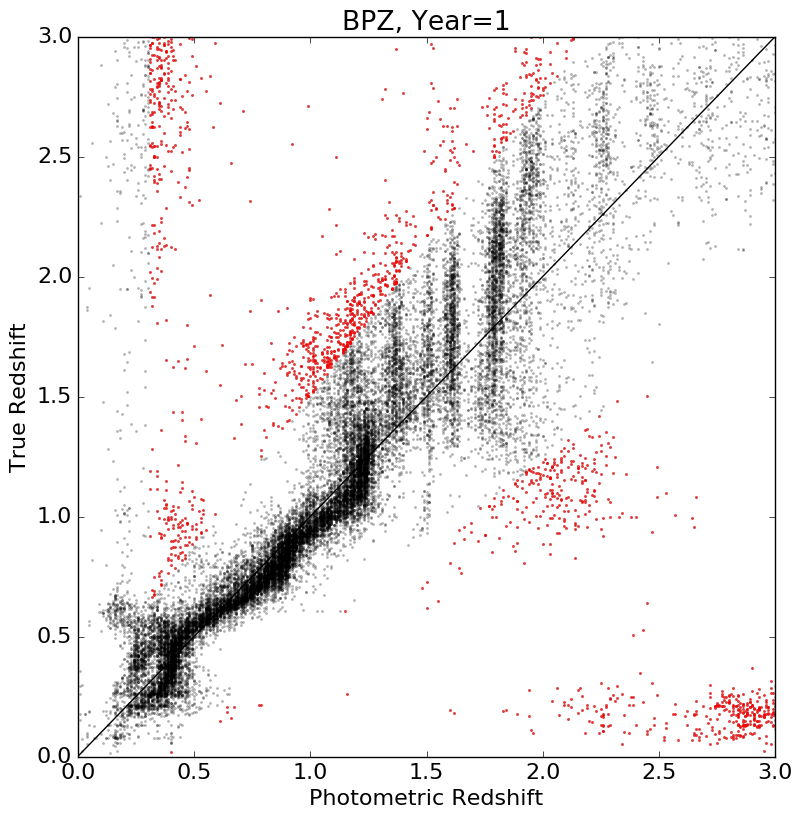
\includegraphics[width=4.0cm]{figures/BPZ_Euclid_Y1_tzpz.png}
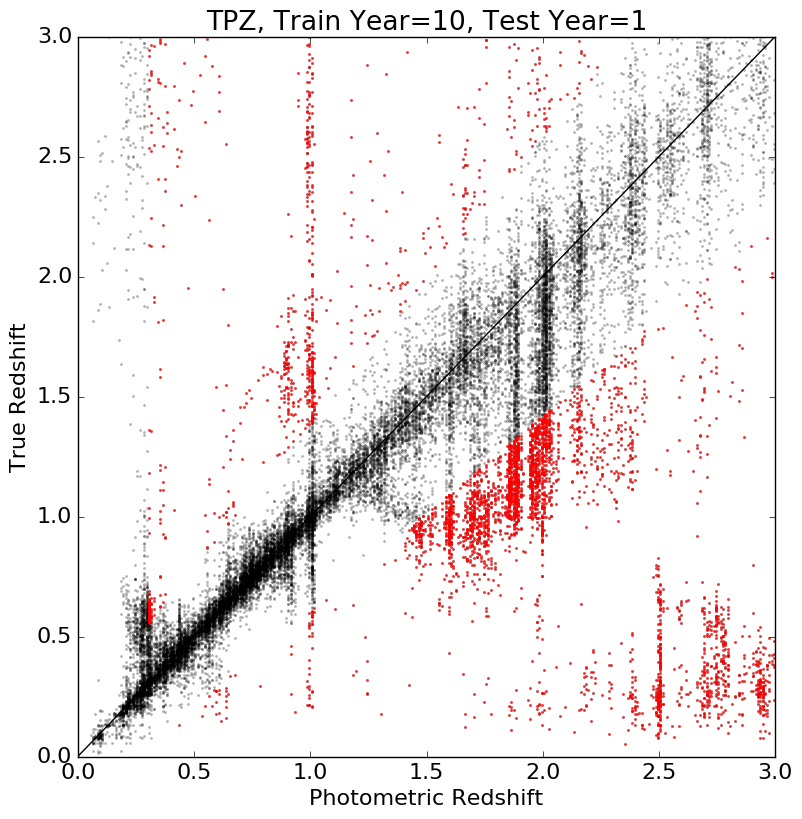
\includegraphics[width=4.0cm]{figures/TPZ_Euclid_10Y1_tzpz.png}
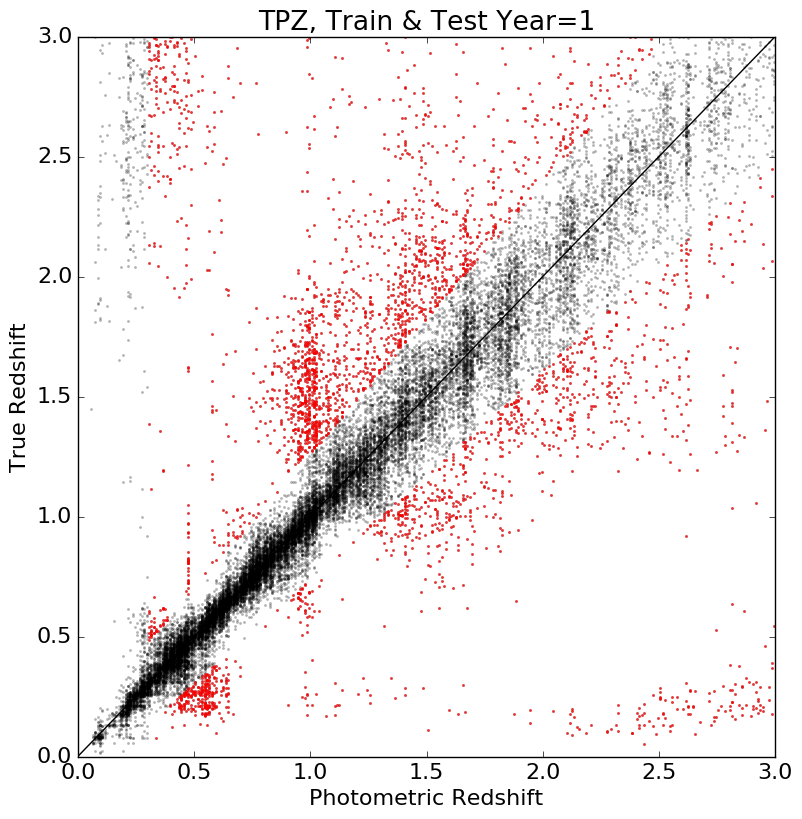
\includegraphics[width=4.0cm]{figures/TPZ_Euclid_1Y1_tzpz.png}
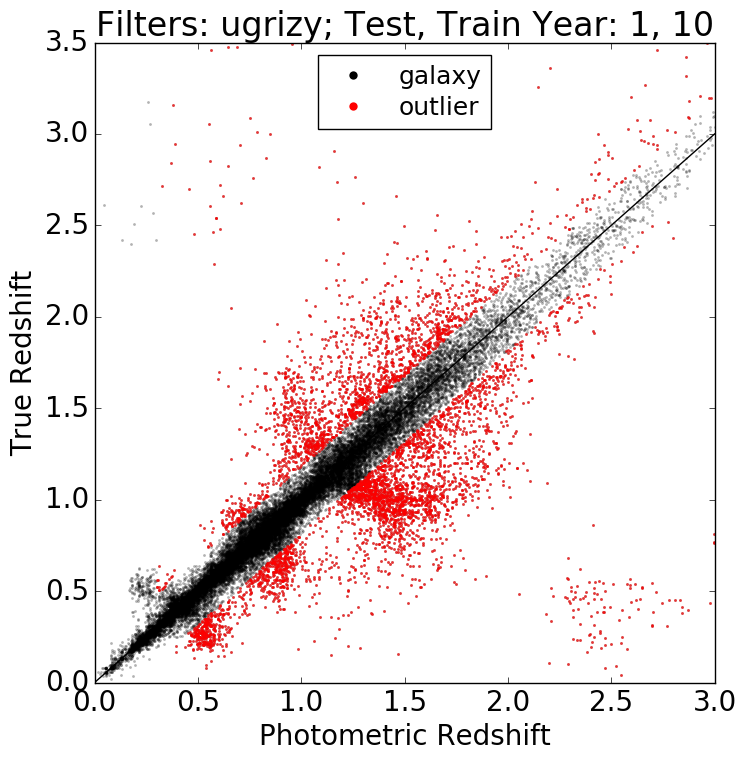
\includegraphics[width=4.0cm]{figures/CM_10Y1_tzpz.png}
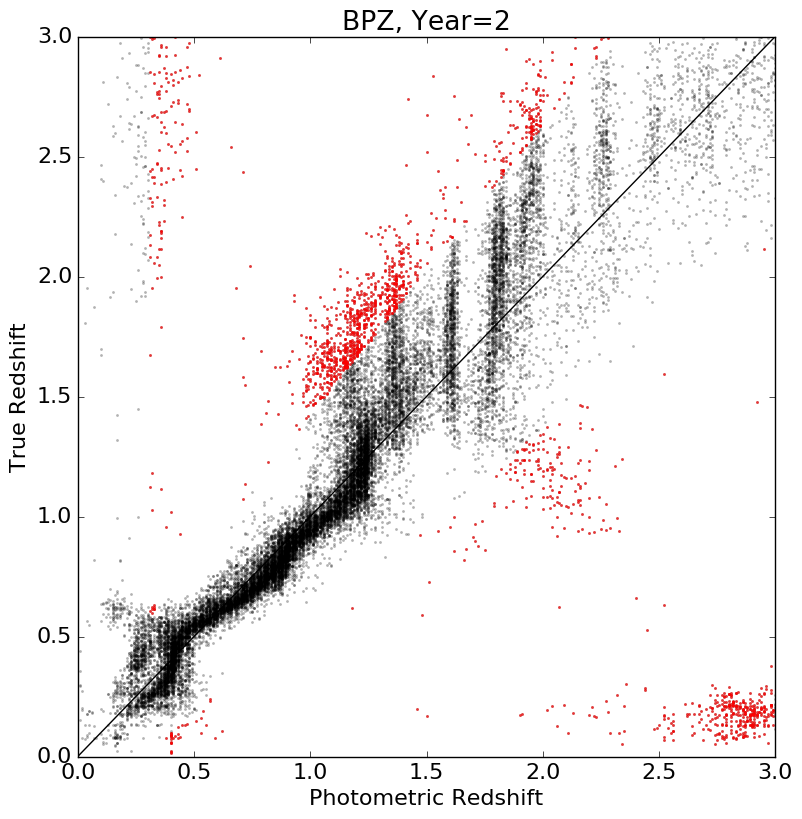
\includegraphics[width=4.0cm]{figures/BPZ_Euclid_Y2_tzpz.png}
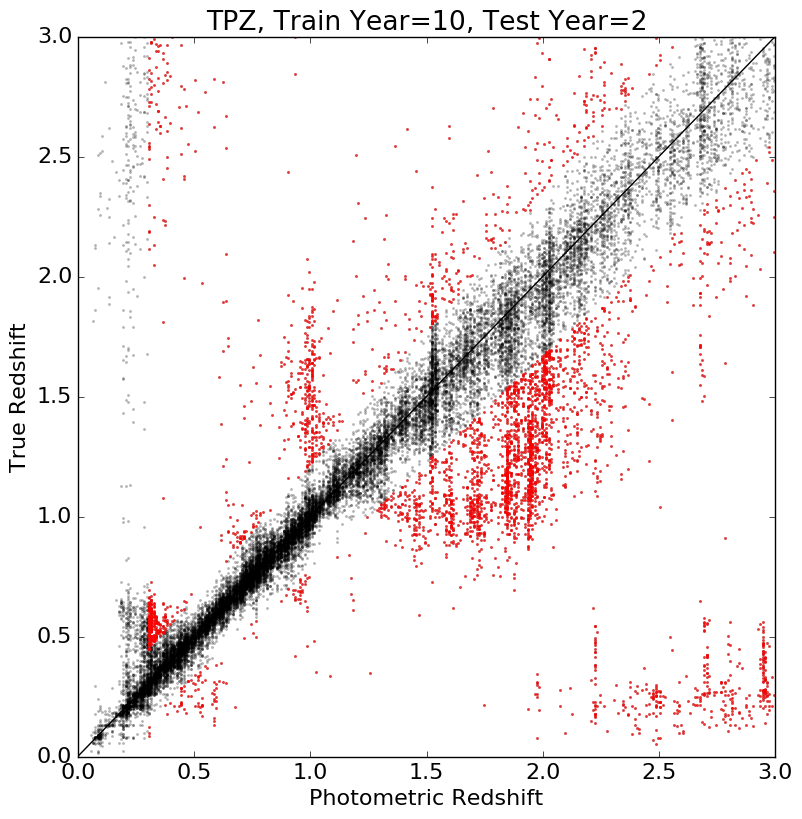
\includegraphics[width=4.0cm]{figures/TPZ_Euclid_10Y2_tzpz.png}
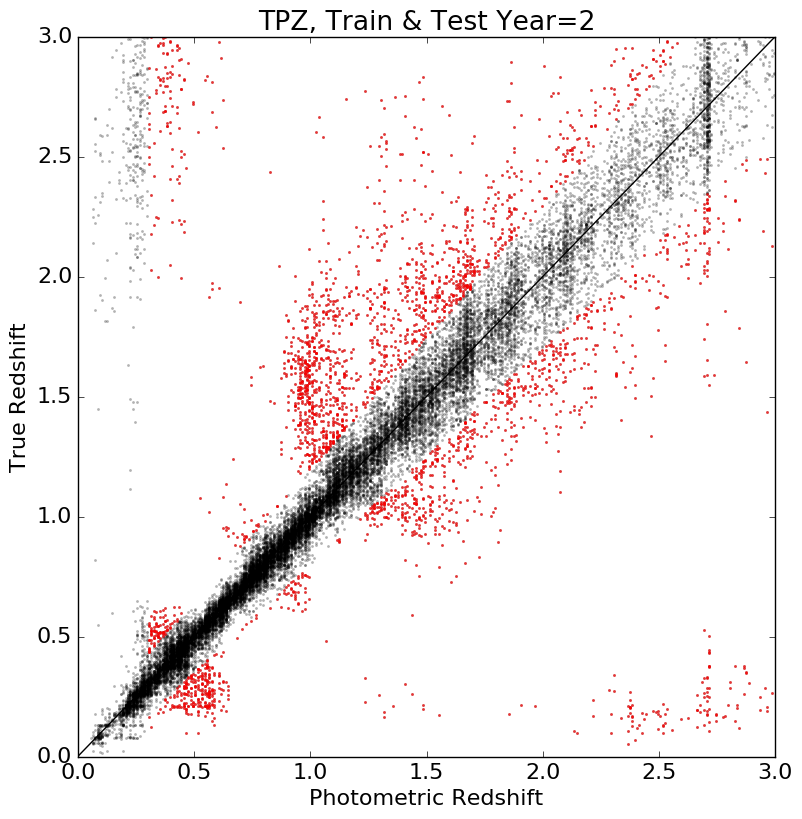
\includegraphics[width=4.0cm]{figures/TPZ_Euclid_2Y2_tzpz.png}
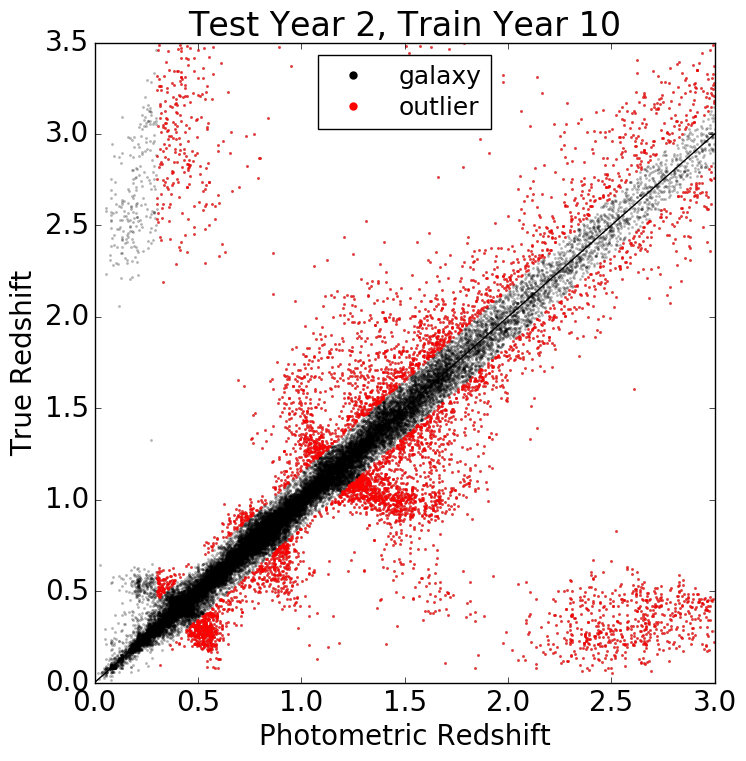
\includegraphics[width=4.0cm]{figures/CM_10Y2_tzpz.png}
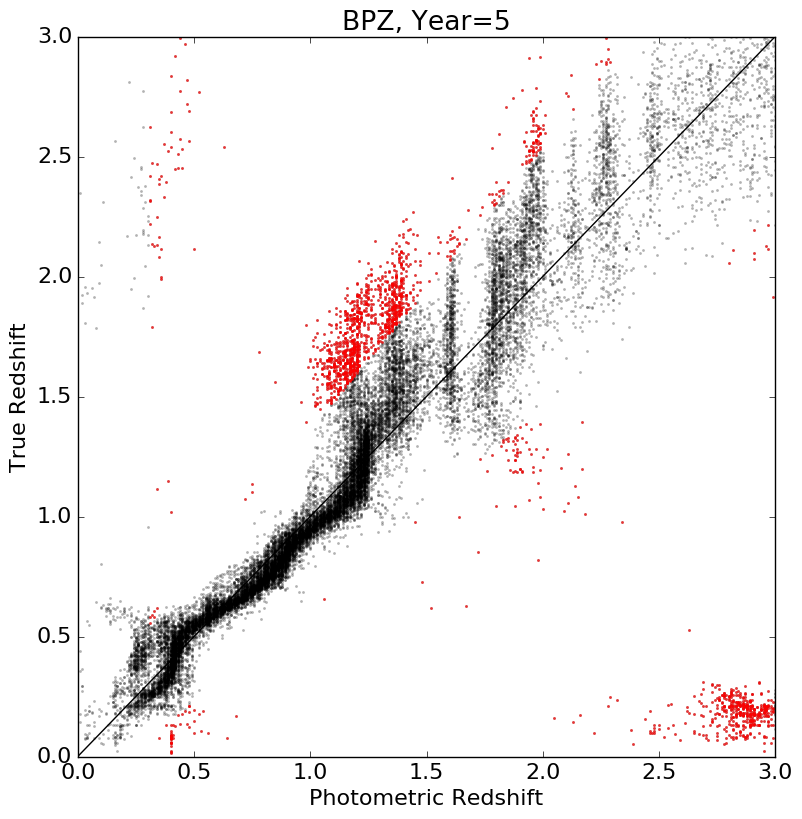
\includegraphics[width=4.0cm]{figures/BPZ_Euclid_Y5_tzpz.png}
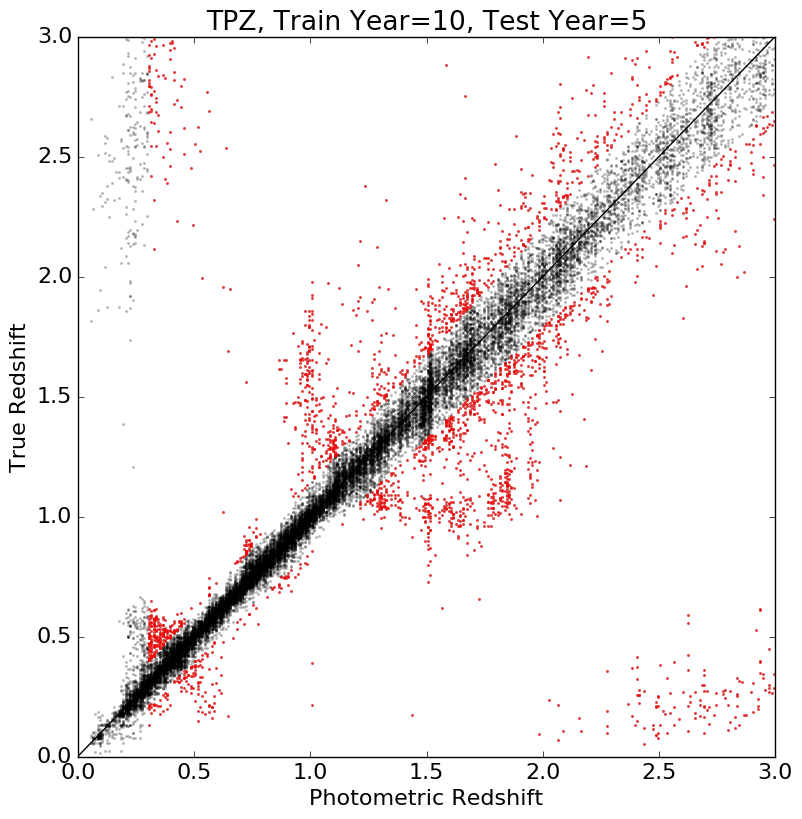
\includegraphics[width=4.0cm]{figures/TPZ_Euclid_10Y5_tzpz.png}
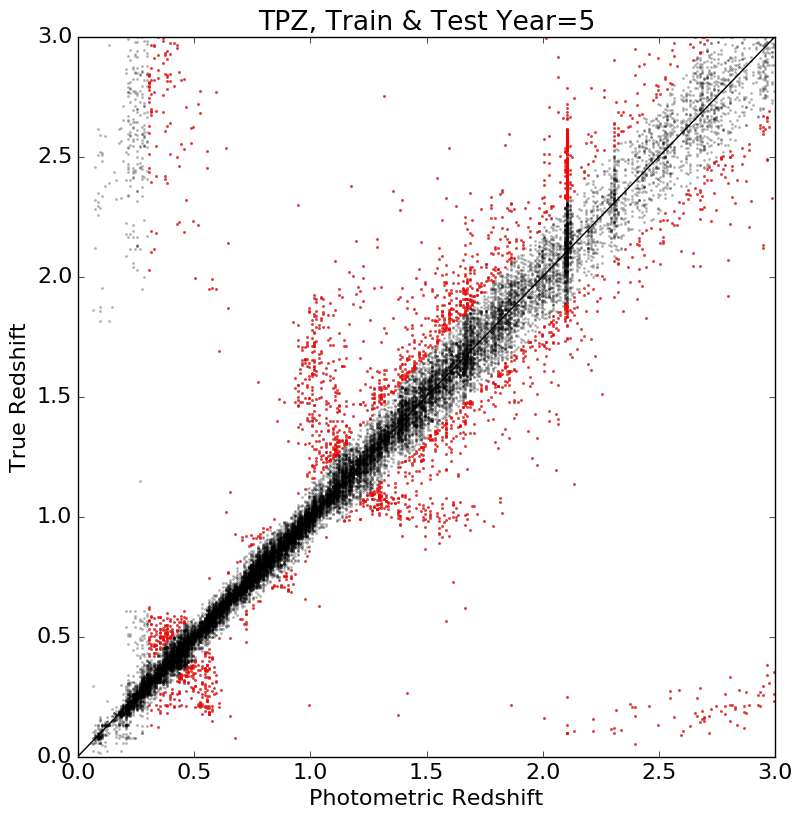
\includegraphics[width=4.0cm]{figures/TPZ_Euclid_5Y5_tzpz.png}
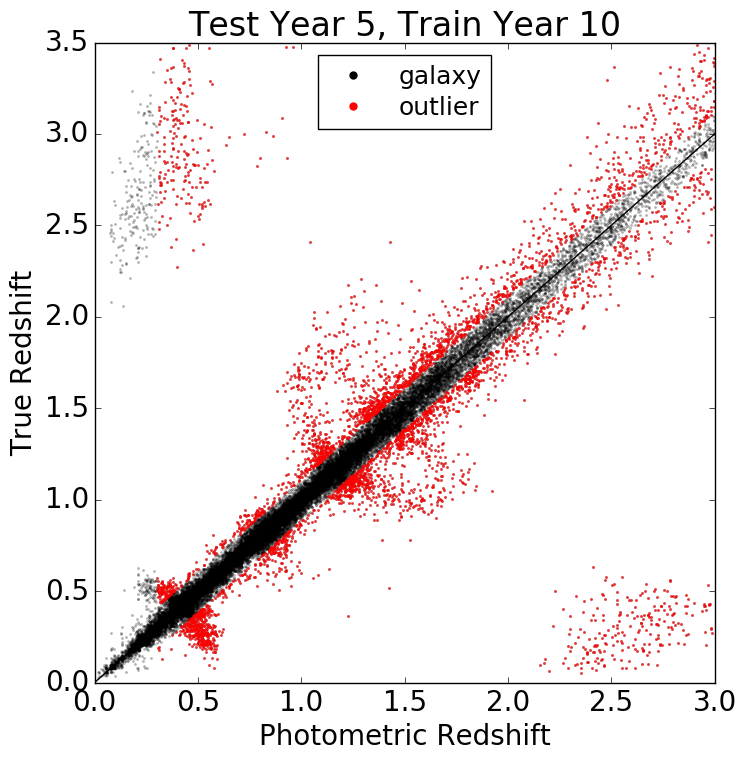
\includegraphics[width=4.0cm]{figures/CM_10Y5_tzpz.png}
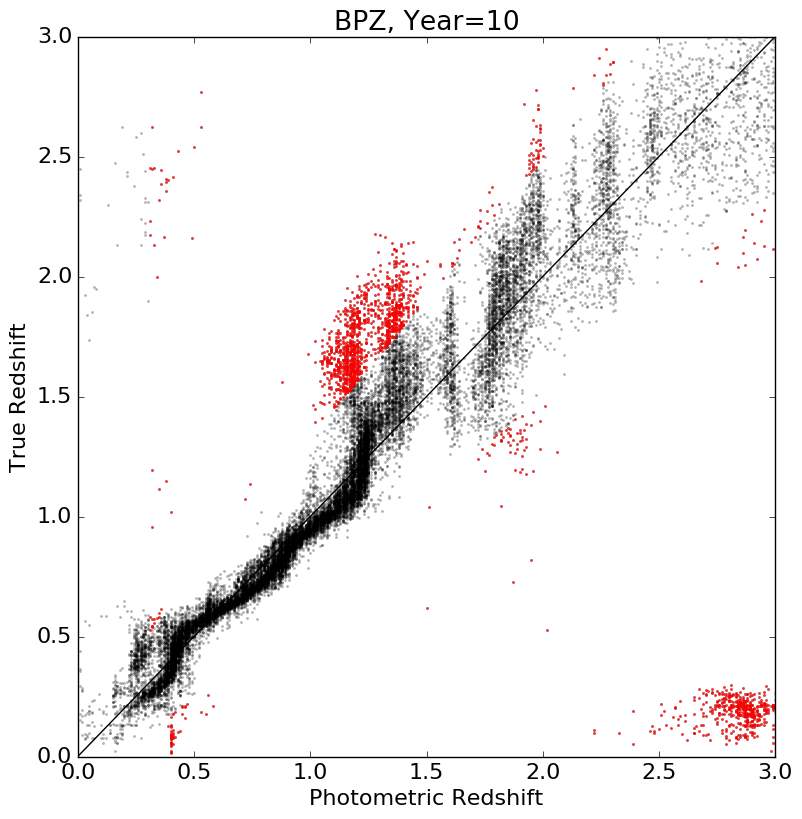
\includegraphics[width=4.0cm]{figures/BPZ_Euclid_Y10_tzpz.png}
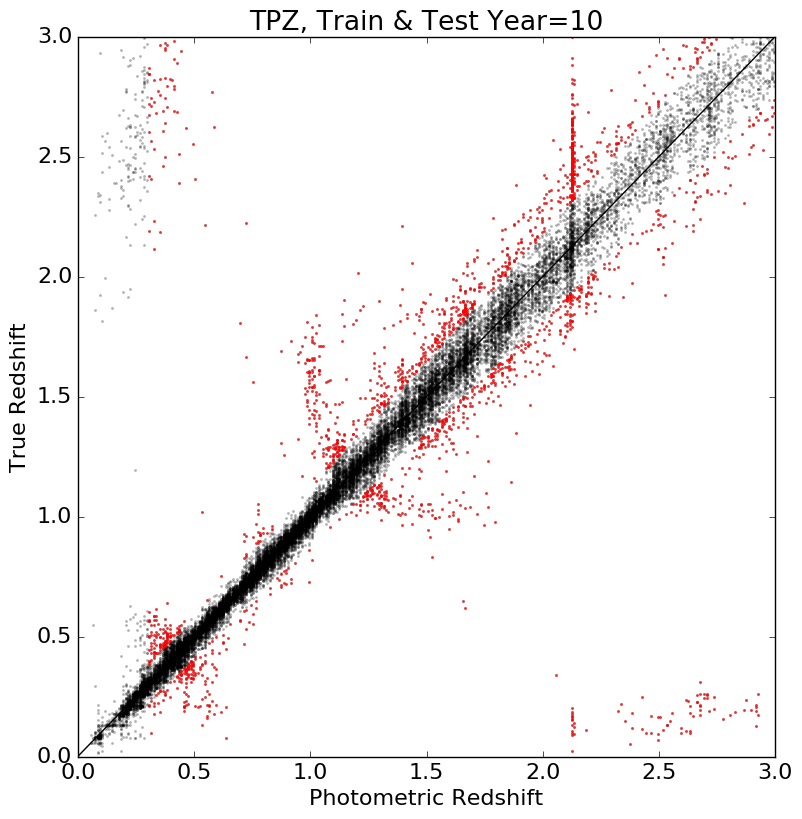
\includegraphics[width=4.0cm]{figures/TPZ_Euclid_10Y10_tzpz.png}
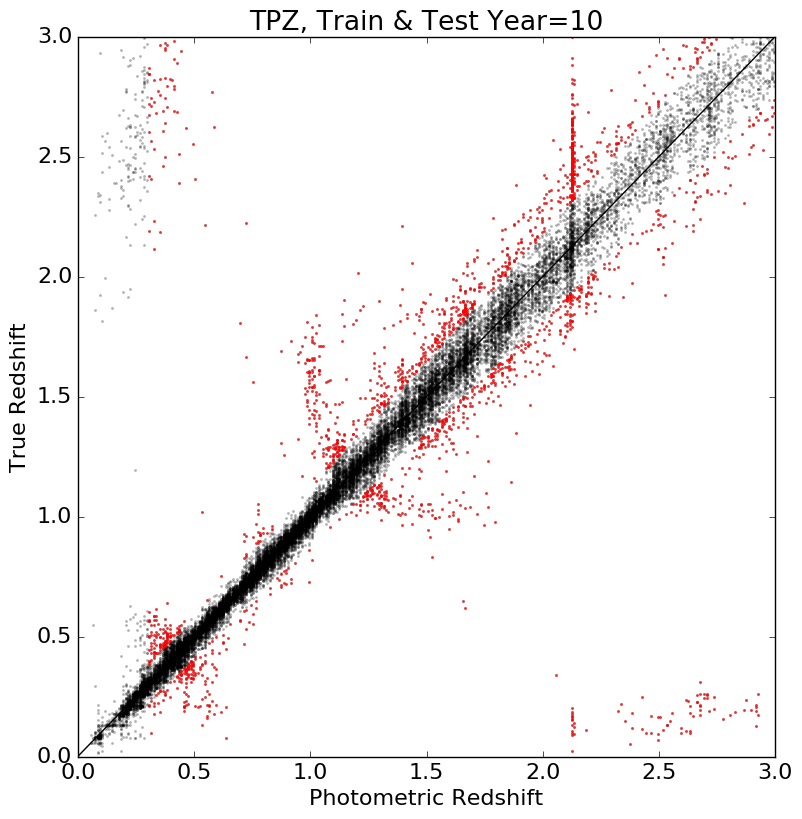
\includegraphics[width=4.0cm]{figures/TPZ_Euclid_10Y10_tzpz.png}
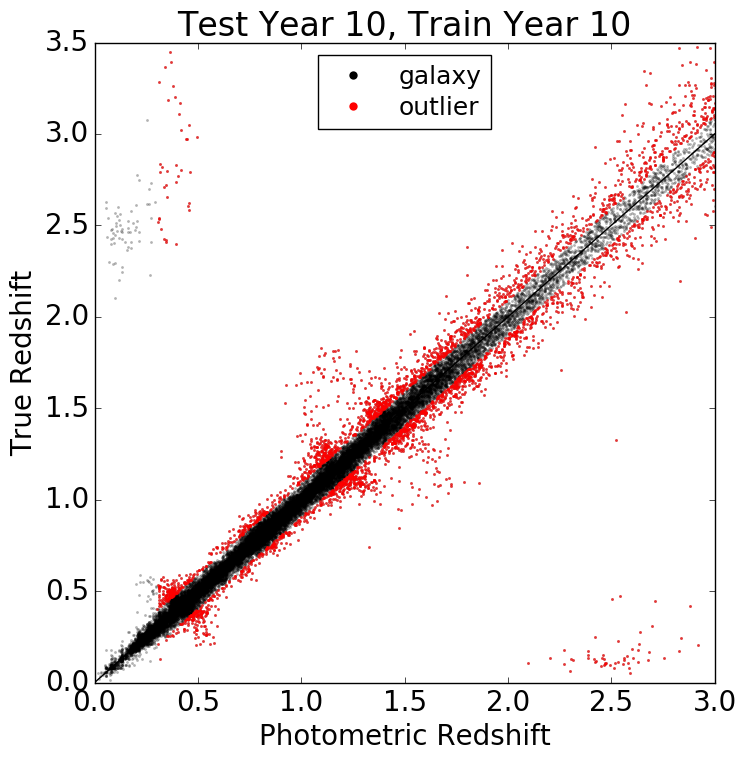
\includegraphics[width=4.0cm]{figures/CM_10Y10_tzpz.png}
\caption{Examples of $z_\mathrm{true}$--$z_\mathrm{phot}$ plots for a variety of algorithms (by column), for 1, 2, 5, or 10 years of survey time elapsed (top to bottom). Galaxies that are statistical outliers are shown in red. \textbf{Left:} results for the BPZ algorithm. \textbf{Center-left:} results for the TPZ algorithm with a 10-year training set. \textbf{Center-right:} results for the TPZ algorithm with a co-evolving training set. \textbf{Right:} results for nearest-neighbors color-matching algorithm, with 50000 test galaxies and $10^6$ training set galaxies with co-evolving photometric errors. \label{fig:tzpz}}
\end{center}
\end{figure*}


\smallskip \noindent \textbf{Statistical Measures} \\
The important statistical measures that are typically used to assess photo-$z$ results are based on the photo-$z$ error, $\Delta z_{(1+z)} = (z_\mathrm{spec}-z_\mathrm{phot})/(1+z_\mathrm{phot}$. We measure the robust standard deviation in $\Delta z_{(1+z)}$, $\sigma_{\Delta z_{(1+z)}}$ (i.e., ``robust'' because it is the standard deviation of galaxies within the IQR); the robust bias, which is the mean deviation $\overline{\Delta z}_{(1+z)}$; and the fraction of outliers, $f_\mathrm{out}$, which is the fraction of galaxies with $|\Delta z_{(1+z)}|> 0.06$ and $>3\sigma_\mathrm{IQR}$ (i.e., must be greater than whichever constraint is larger). In the community sometimes the median deviation in $\Delta z_{(1+z)}$ over all galaxies is used instead of the mean deviation of galaxies within the IQR, but we find the two are comparable. In Figure \ref{fig:stats} we demonstrate a convenient way to statistically compare the results from multiple photo-$z$ estimators. In this case we are comparing the values of these statistical measures when the photo-$z$ estimators are run on galaxy catalogs simulated to represent the 1, 2, 5, and 10 year DRP from LSST (colored lines), for both BPZ (left) and TPZ (right). Different estimators for the same year could also be plotted in a single graph. From these statistical measures it is obvious, for example, that the photo-$z$ from TPZ outperform those from BPZ at all years. In Figure \ref{fig:stat_stat} we show examples of how to compare the statistical measures for the full catalog (i.e., $0.3 \leq z_\mathrm{phot} \leq 3.0$) for different photo-$z$ estimators by plotting, e.g., the fractions of failures versus the outliers, or the bias versus the standard deviation.

\begin{figure*}
\begin{center}
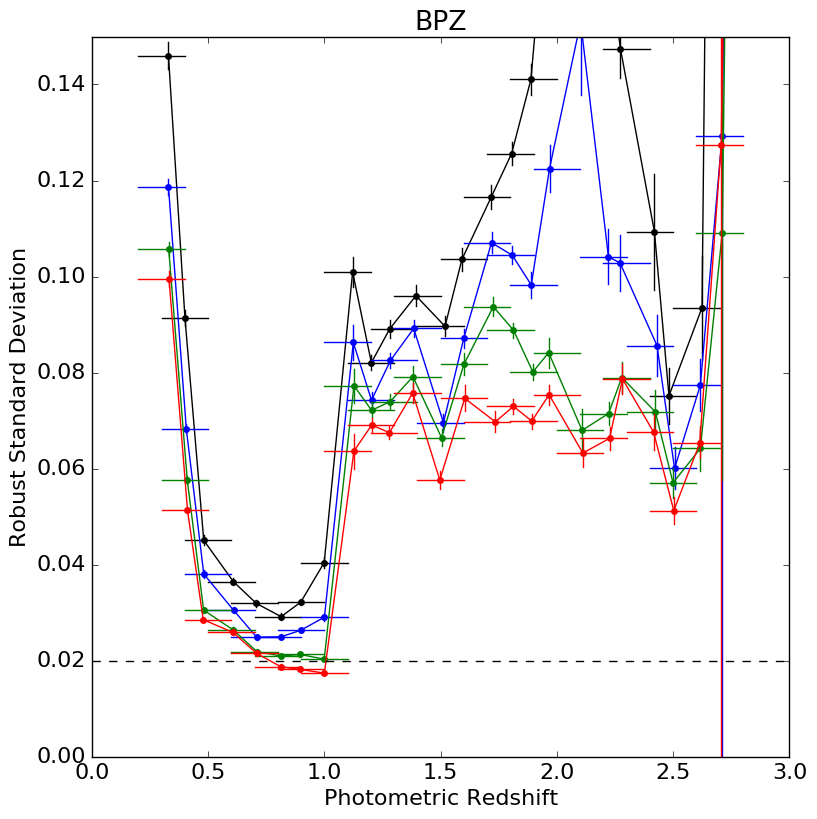
\includegraphics[width=6cm]{figures/BPZ_Euclid_IQRs.png}
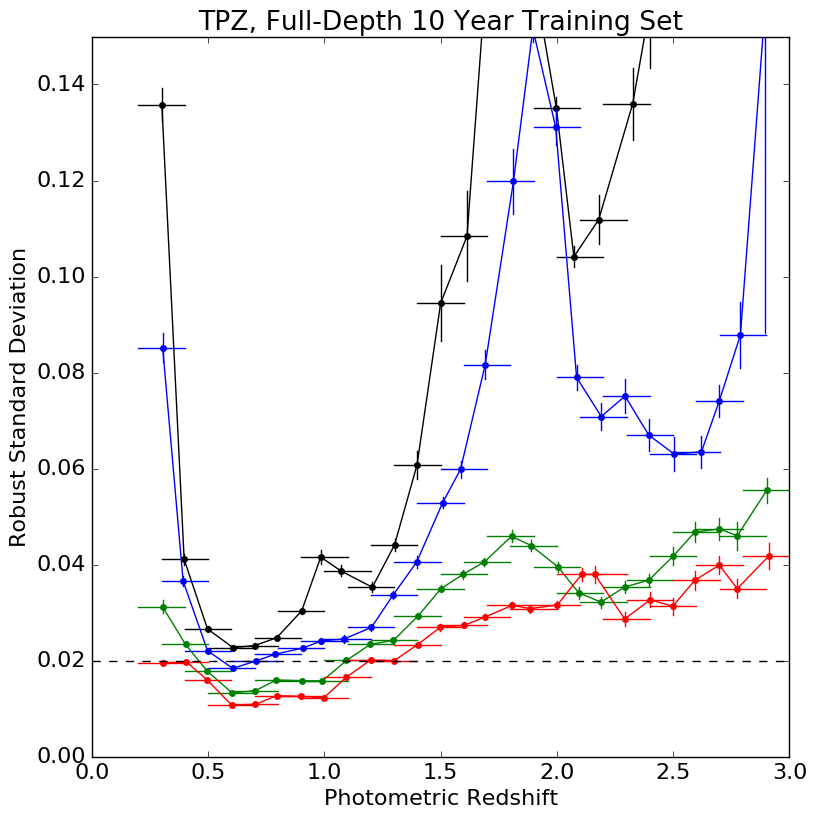
\includegraphics[width=6cm]{figures/TPZ_Euclid_TFD_IQRs.png}
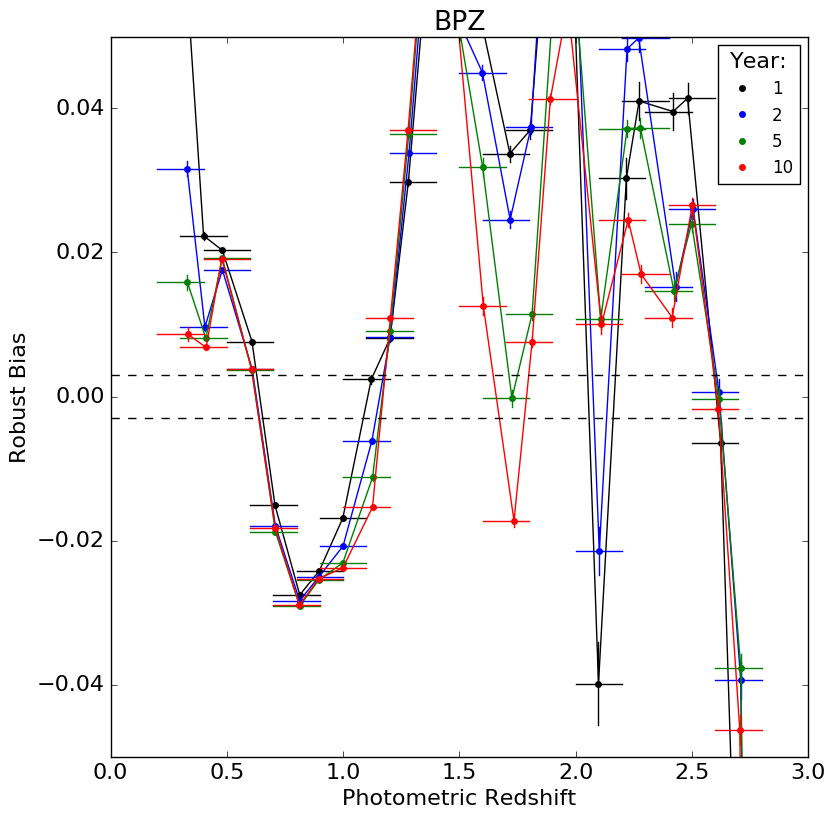
\includegraphics[width=6cm]{figures/BPZ_Euclid_bias.png}
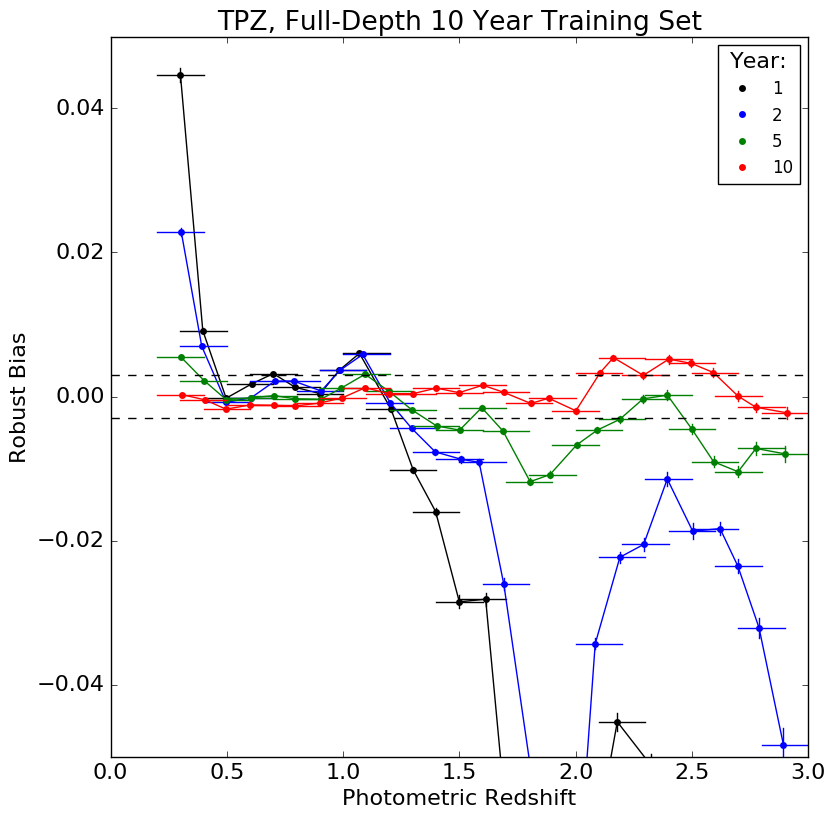
\includegraphics[width=6cm]{figures/TPZ_Euclid_TFD_bias.png}
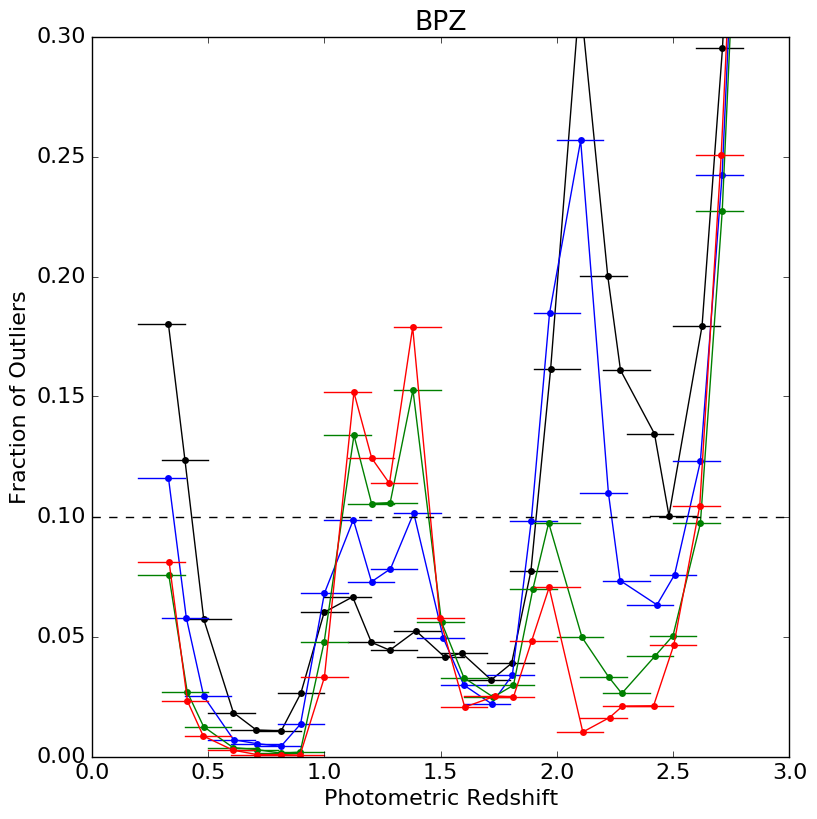
\includegraphics[width=6cm]{figures/BPZ_Euclid_fout.png}
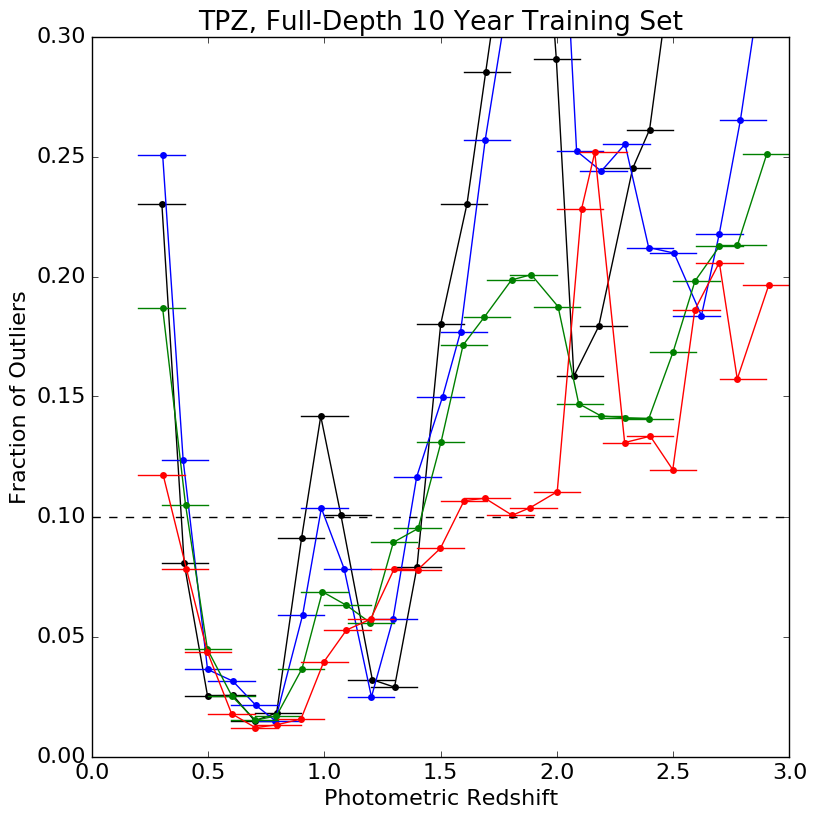
\includegraphics[width=6cm]{figures/TPZ_Euclid_TFD_fout.png}
\caption{Examples of a statistical measures of the photo-$z$ results from BPZ (left) and TPZ with an evolving training set (right) for simulated catalogs at 1 to 10 years (line colors as in plot legends). From top to bottom we show the robust standard deviation from the IQR, the robust bias, and the fraction of outliers as a function of photo-$z$, with matched $x$- and $y$-axes to facilitate comparison between BPZ and TPZ. \label{fig:stats}}
\end{center}
\end{figure*}

\begin{figure*}
\begin{center}
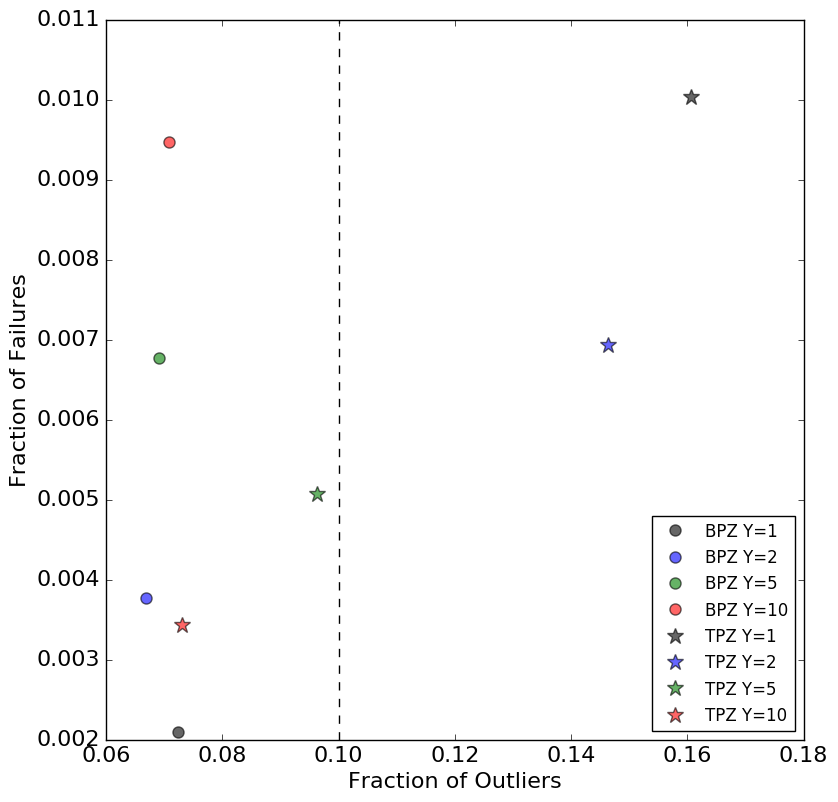
\includegraphics[width=8cm]{figures/stat_stat_fout_ffail.png}
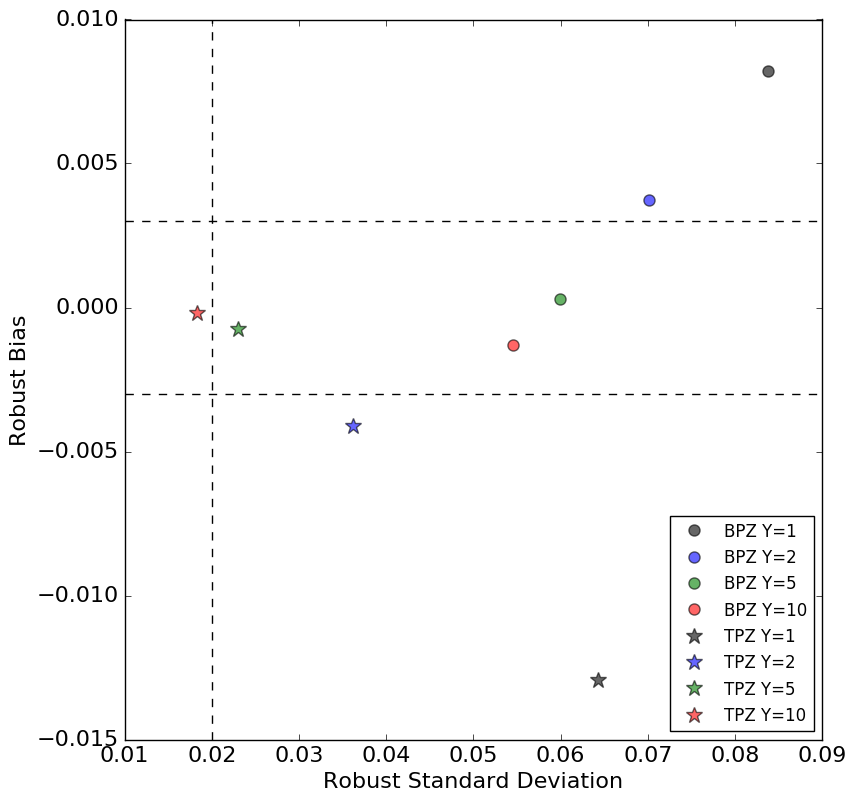
\includegraphics[width=8cm]{figures/stat_stat_std_bias.png}
\caption{Examples of how to compare statistical measures over $0.3 \leq z_\mathrm{phot} \leq 3.0$ from different photo-$z$ estimators by plotting one against the other: fraction of failures and outliers (left), and the robust bias and standard deviation (right). In this case we're comparing the statistical measures for TPZ and BPZ from photometry simulated for the LSST at years 1, 2, 5, and 10 (legend).  \label{fig:stat_stat}}
\end{center}
\end{figure*}


\smallskip \noindent \textbf{Photo-$z$ Uncertainties, $\delta z_\mathrm{phot}$} \\
In Figure \ref{fig:pzpze} we demonstrate a way to assess the photo-$z$ uncertainties, $\delta z_\mathrm{phot}$, that come out of the estimators: we plot $z_\mathrm{phot}$--$\delta z_\mathrm{phot}$ in the main axis, and above and to the side plot the distributions in $\delta z_\mathrm{phot}$, $z_\mathrm{phot}$, and for comparison, $z_\mathrm{true}$. With BPZ, we can see a strict floor in the photo-$z$ uncertainty that increases with redshift (i.e., the uncertainties are bogus, though this could be a fault of mine in running the code and not of the code itself). For both BPZ and TPZ we can see that in some cases the clumps causing a quantization in photo-$z$ also have high photo-$z$ uncertainty, suggesting that a simple cut on $\delta z_\mathrm{phot}$ could return a sample for which the photo-$z$ distribution matches the true distribution. However, there are other clumps in photo-$z$ that have a relatively low uncertainty. Overall, from these plots we could conclude that the TPZ algorithm returns a redshift distribution that is more similar to the true distribution. Another option here is to plot the photo-$z$ error ($\Delta z_{(1+z)}$).

\begin{figure*}
\begin{center}
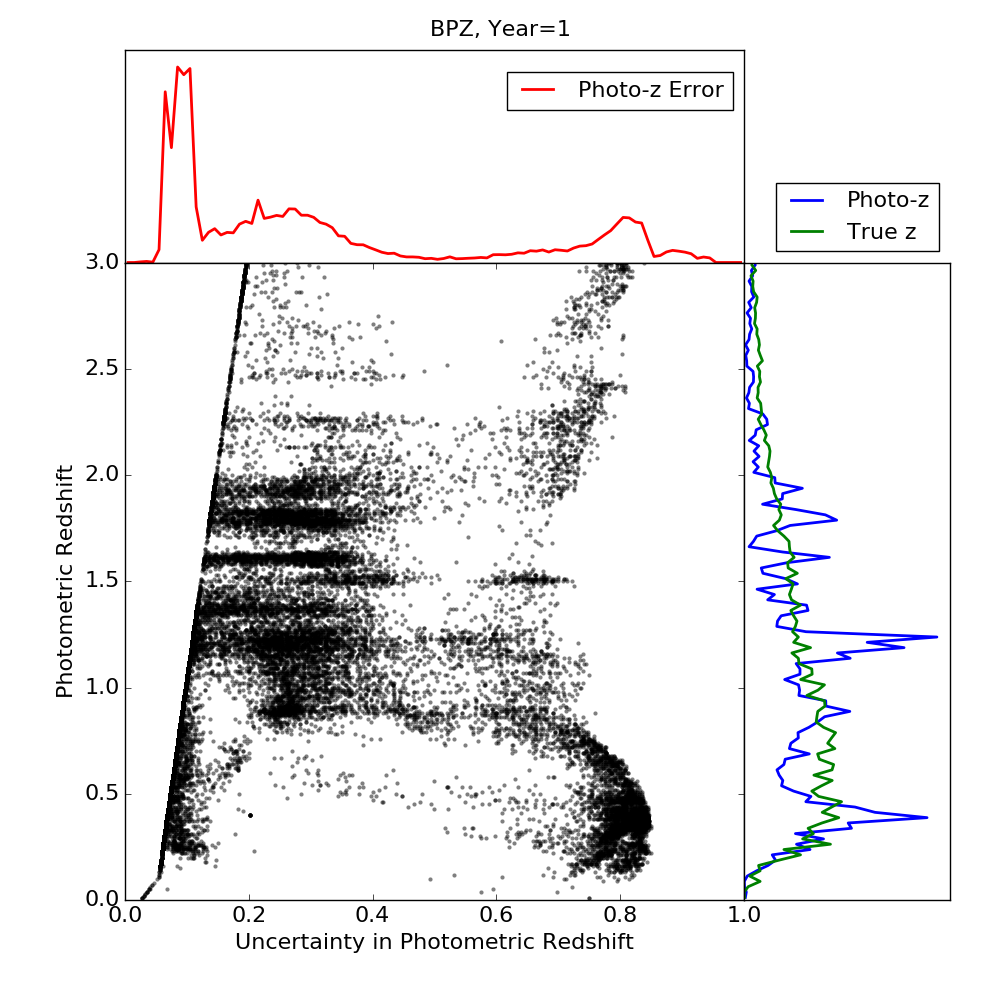
\includegraphics[width=6cm,trim={1cm 1cm 1cm 0cm}, clip]{figures/zp_zpe_bpz_euclid_1_2.png}
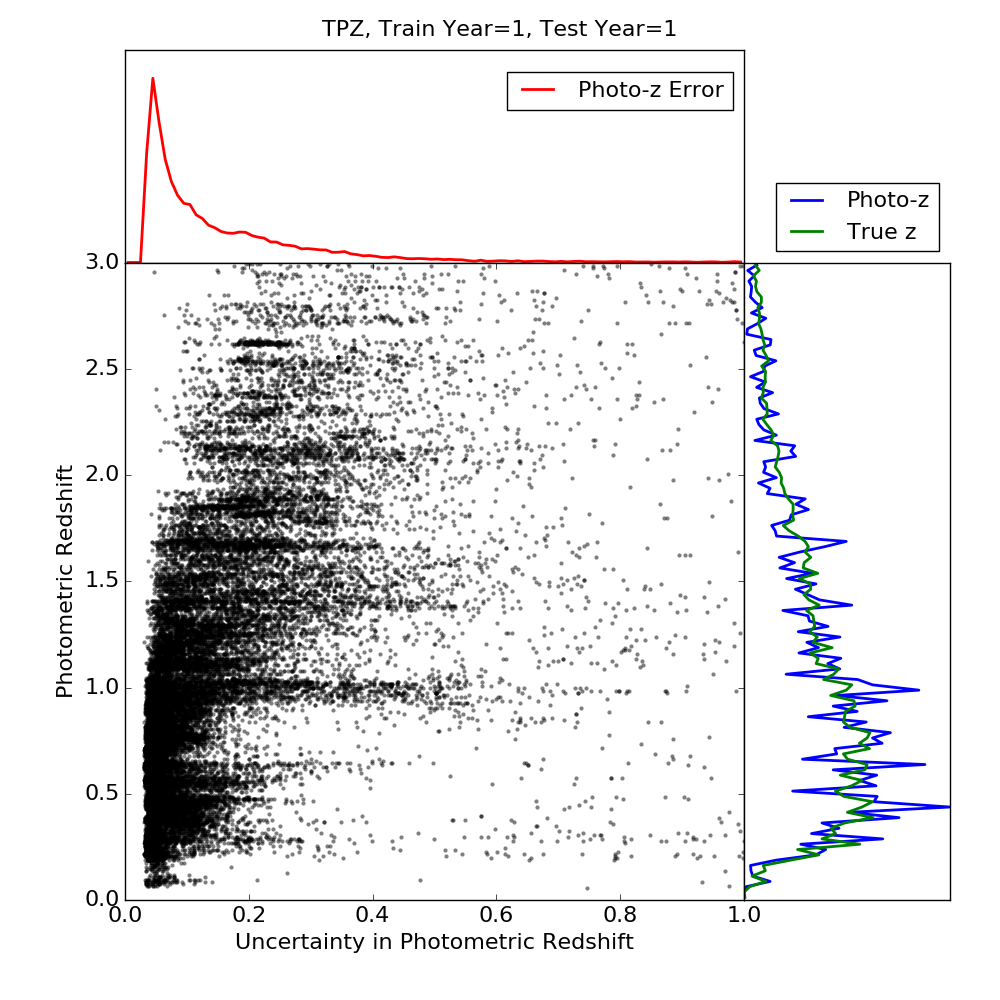
\includegraphics[width=6cm,trim={1cm 1cm 1cm 0cm}, clip]{figures/zp_zpe_tpz_euclid_1_1_2.png}
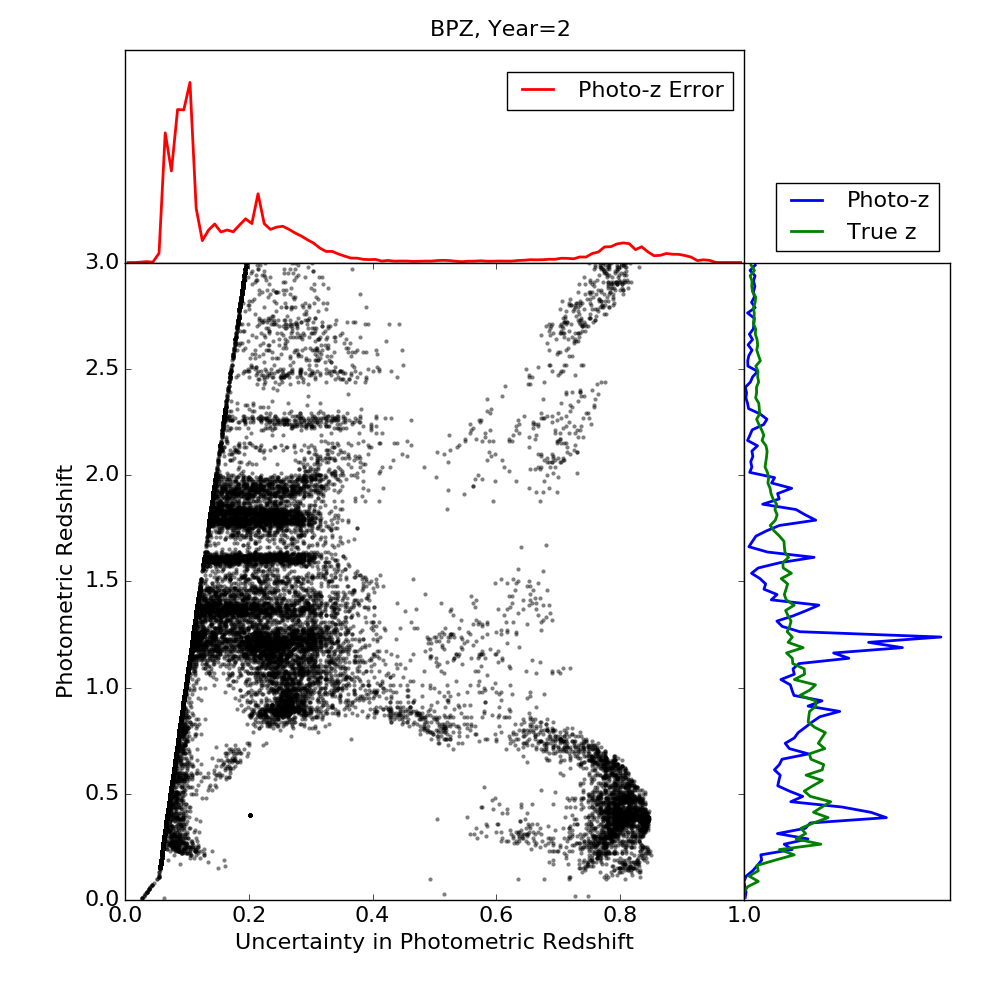
\includegraphics[width=6cm,trim={1cm 1cm 1cm 0cm}, clip]{figures/zp_zpe_bpz_euclid_2_2.png}
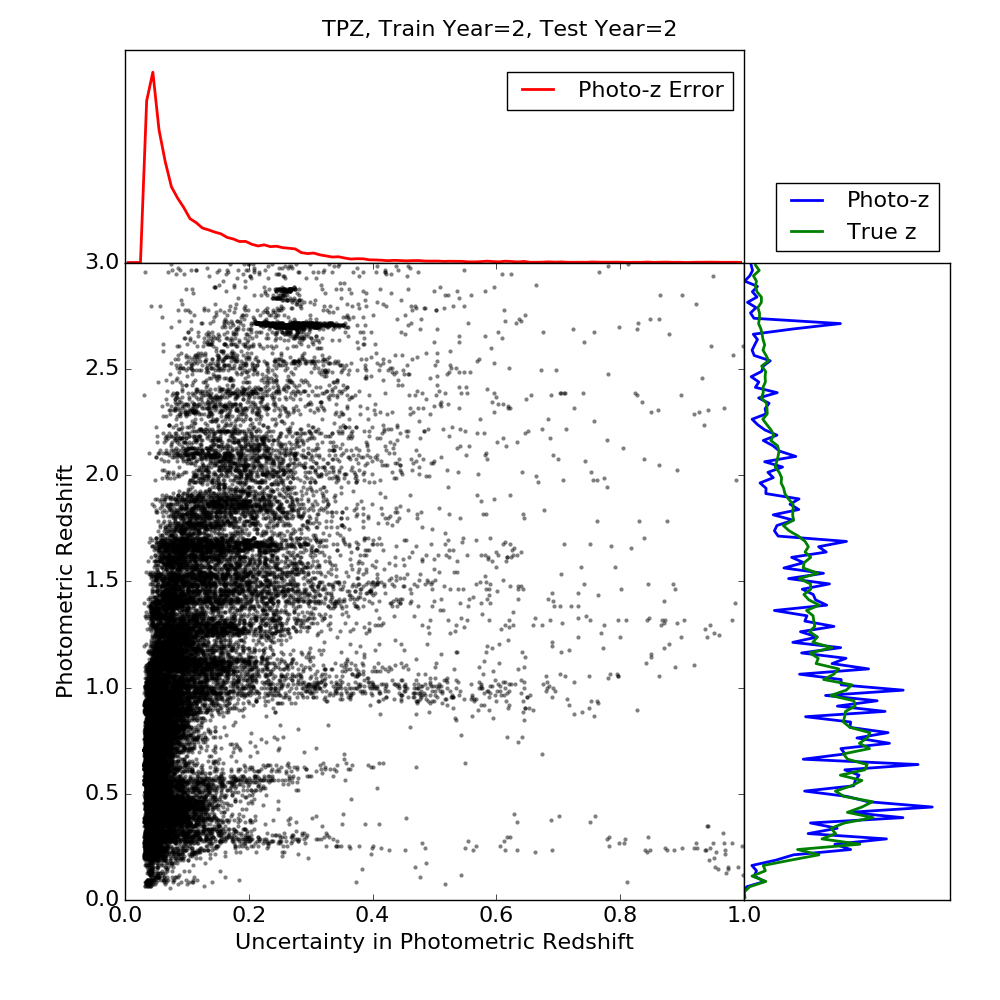
\includegraphics[width=6cm,trim={1cm 1cm 1cm 0cm}, clip]{figures/zp_zpe_tpz_euclid_2_2_2.png}
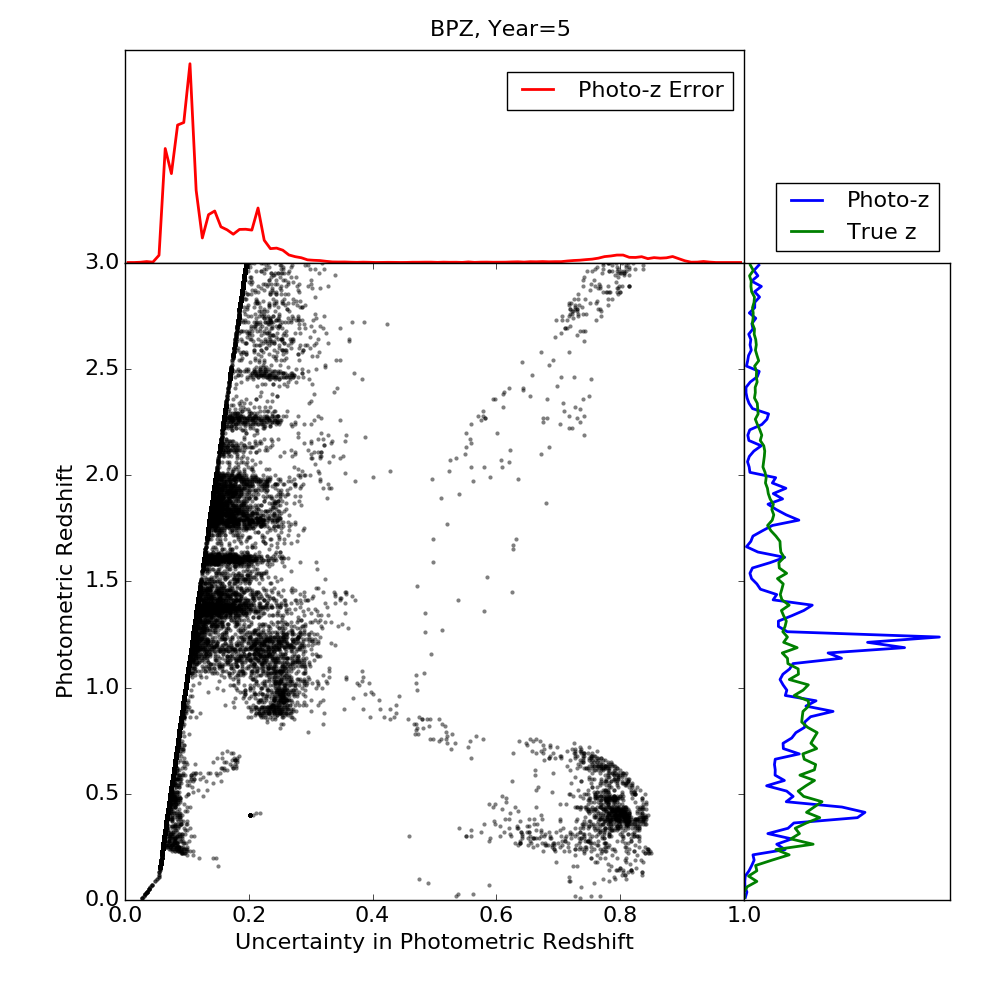
\includegraphics[width=6cm,trim={1cm 1cm 1cm 0cm}, clip]{figures/zp_zpe_bpz_euclid_5_2.png}
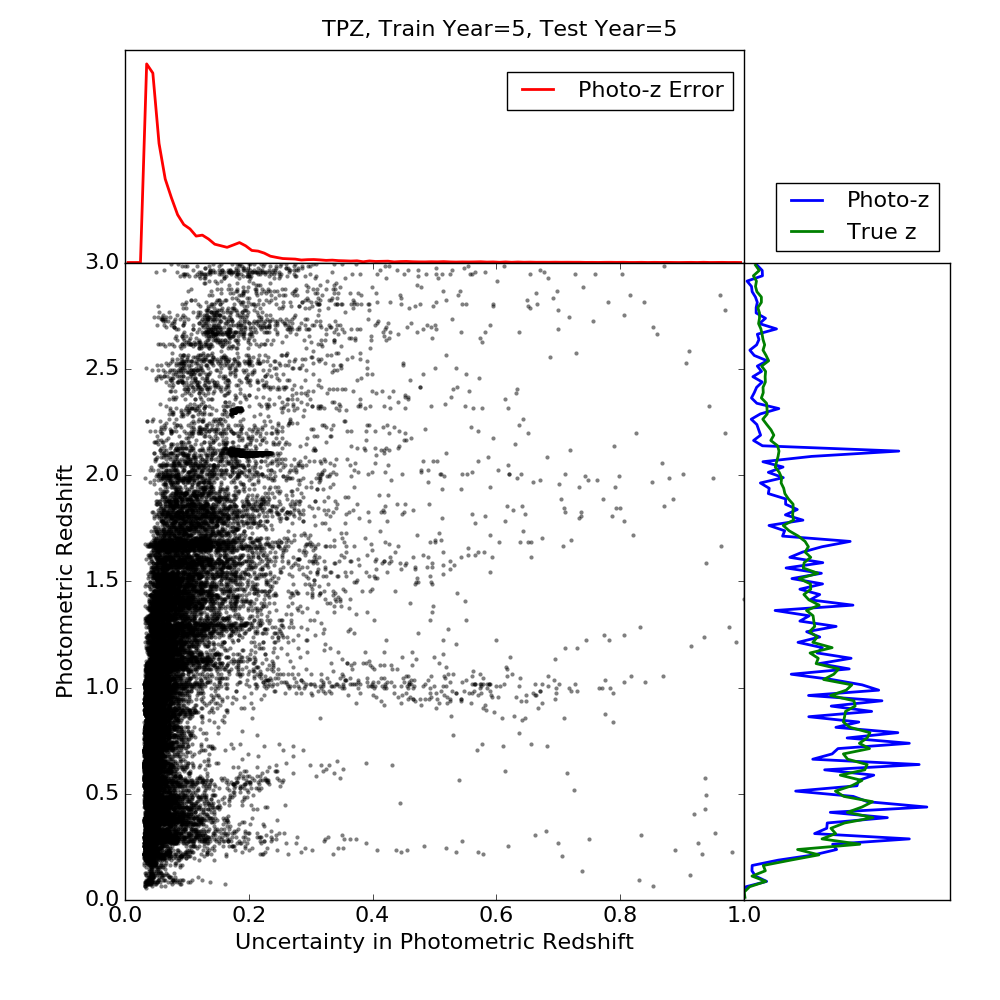
\includegraphics[width=6cm,trim={1cm 1cm 1cm 0cm}, clip]{figures/zp_zpe_tpz_euclid_5_5_2.png}
\caption{Examples of plot to compare the photo-$z$ uncertainty ($\delta z_\mathrm{phot}$) between algorithms with $z_\mathrm{phot}$--$\delta z_\mathrm{phot}$ plots from the BPZ (left) and TPZ (right) estimators for simulated catalogs with photometric uncertainties at 1, 2, and 5 years of LSST (top to bottom). Red lines show the distribution of photo-$z$ errors; blue and green lines compare the distributions of true and photometric redshifts. \label{fig:pzpze}}
\end{center}
\end{figure*}


\smallskip \noindent \textbf{The Posterior Probability Density Function, $P(z)$} \\
In Figure \ref{fig:zpdf} we plot examples of the posterior probability density functions output by the BPZ and TPZ algorithms for two test galaxies. One galaxy was chosen as a random representative of galaxies for which an inaccurate and imprecise photo-$z$ was returned from both BPZ and TPZ for all years (top panel of Figure \ref{fig:zpdf}). The other was chosen as a random representative of galaxies which experienced a large and consistent improvement in both the accuracy and precision of its photo-$z$ from year 1 to 10, for both BPZ and TPZ (bottom panel of Figure \ref{fig:zpdf}). These kind of plots demonstrate, for example, the quantization in the TPZ photo-$z$ in the PDFs (this may be related to a mistake in the TPZ input).

\begin{figure*}
\begin{center}
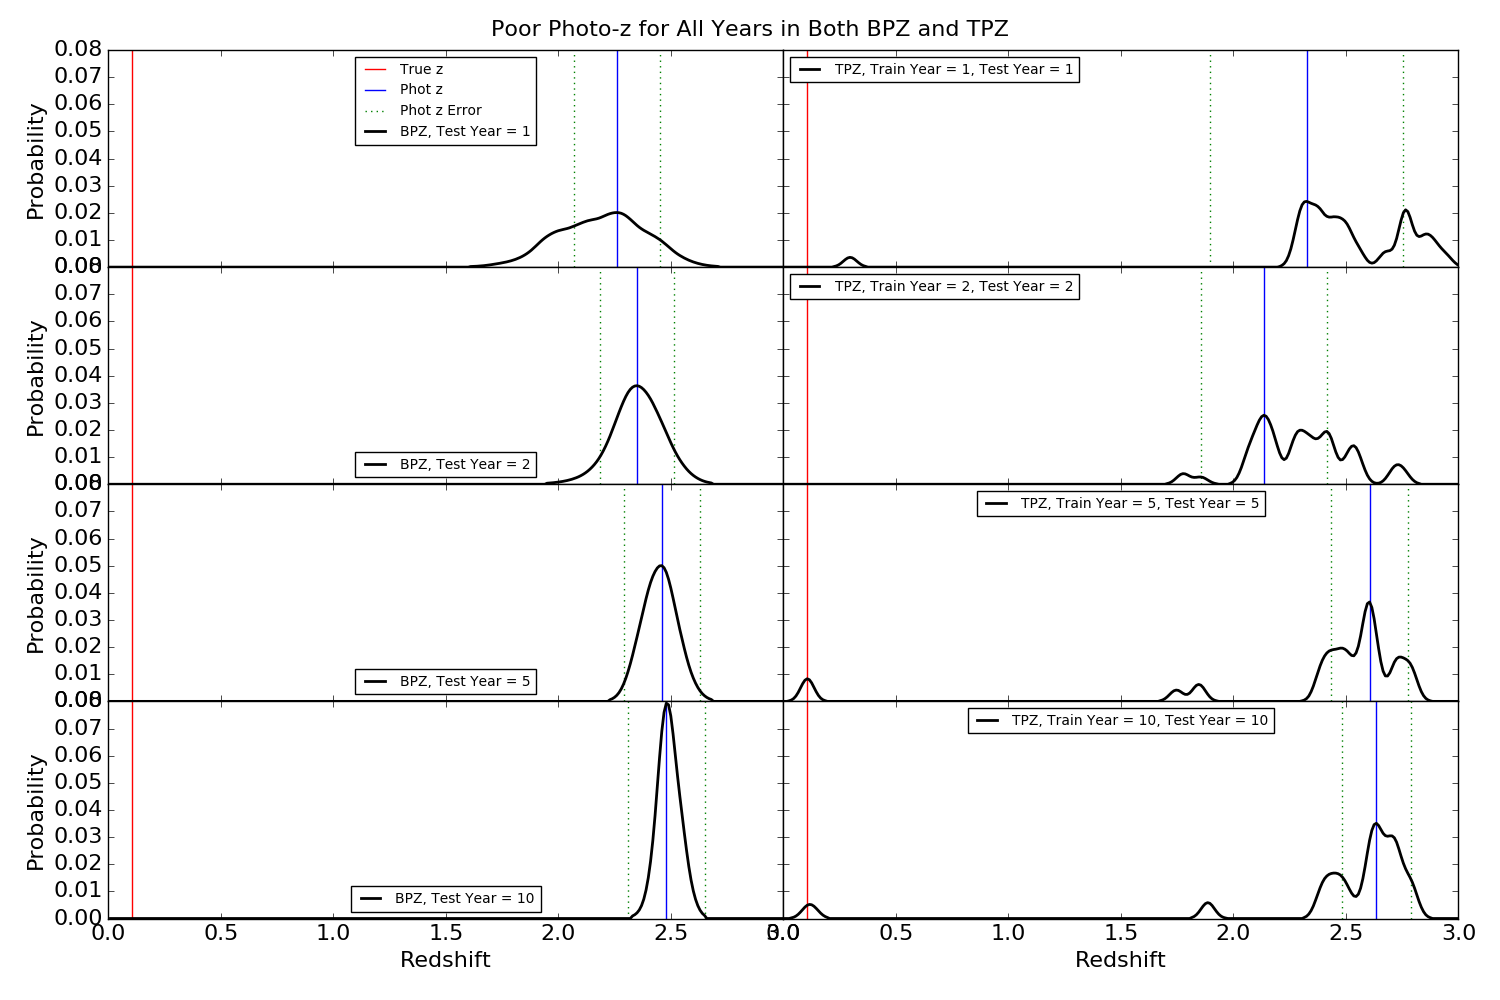
\includegraphics[width=13cm]{figures/zpdf_g4.png}
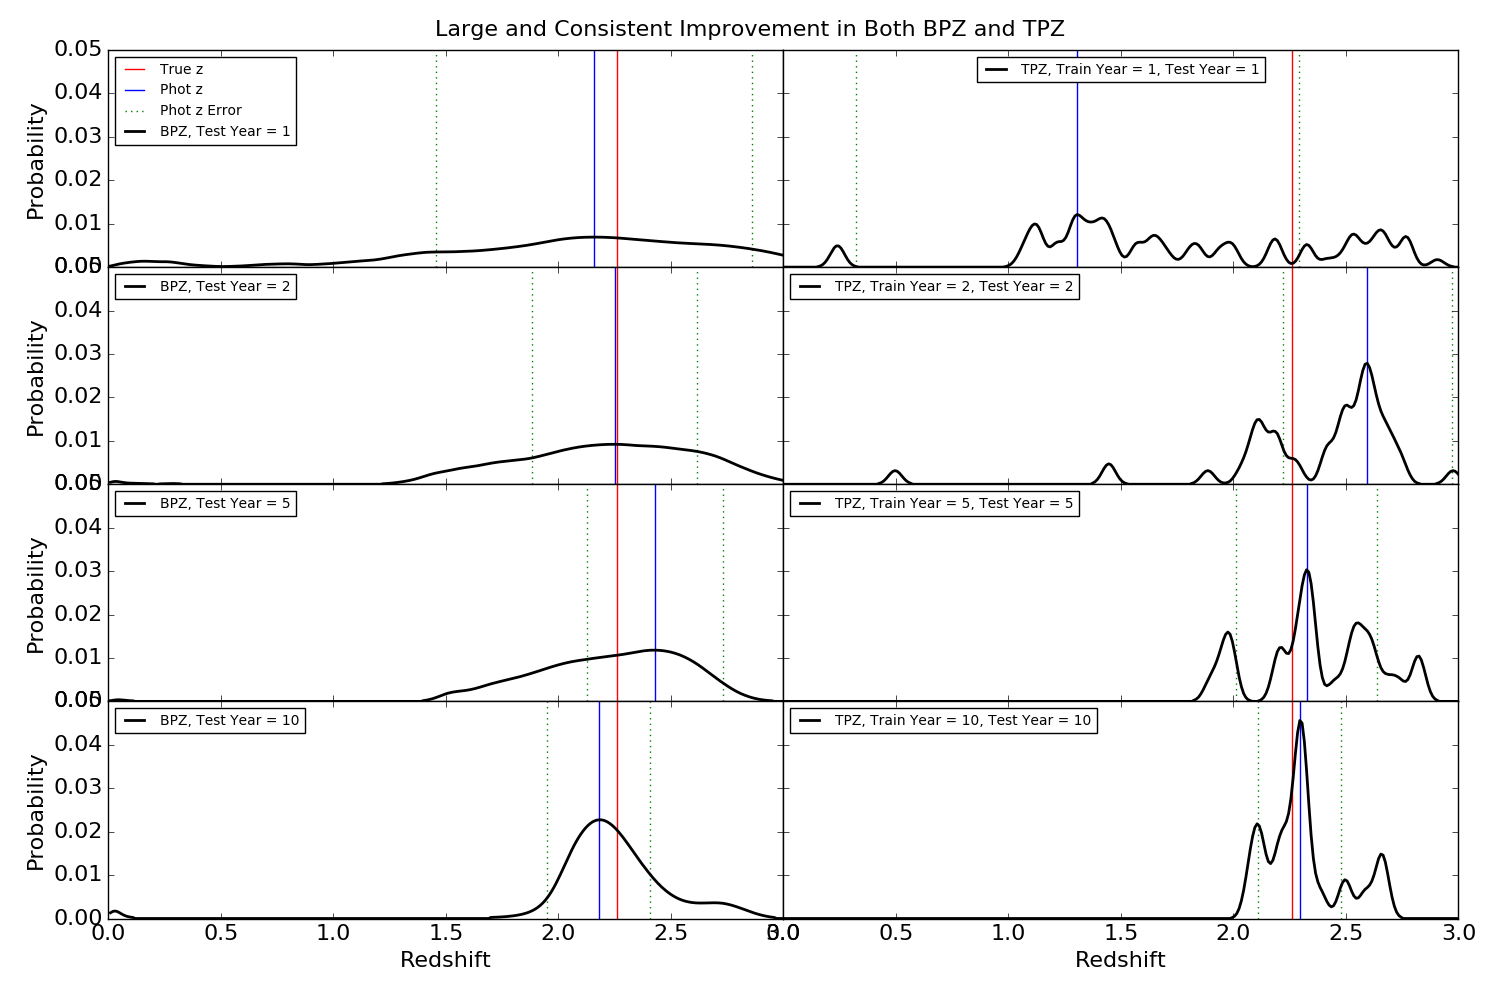
\includegraphics[width=13cm]{figures/zpdf_g7.png}
\caption{Examples of the posterior probability density functions for two test galaxies in all of our simulations: BPZ (left) and TPZ (right) for photometric uncertainties like 1, 2, 5, and 10 years of LSST (rows from top to bottom). In the top panel we choose a galaxy that return inaccurate and imprecise photo-$z$ from all 8 trials, and in the bottom panel we choose a galaxy that experienced a large and consistent improvement in photo-$z$ accuracy and precision from 1 to 10 years with both estimators.  \label{fig:zpdf}}
\end{center}
\end{figure*}

\smallskip \noindent \textbf{Q-Q Plots} \\
In Figure \ref{fig:qq} we show an example of a quantile-quantile plot using the true $vs.$ the photometric redshift. Each point represents the $z_\mathrm{true}$ and $z_\mathrm{phot}$ for a given quantile, and since the two distributions we are comparing have the same total number of objects (we've neglected any galaxies that have failed to return a photo-$z$), we're simply using $1/N$ as the quantiles. If the Q-Q plot is linear with a slope of 1, we would know the distributions of $z_\mathrm{phot}$ would match that of $z_\mathrm{true}$. In Figure \ref{fig:qq} we can see for both BPZ and TPZ that this is not the case, but that BPZ is worse.

\begin{figure*}
\begin{center}
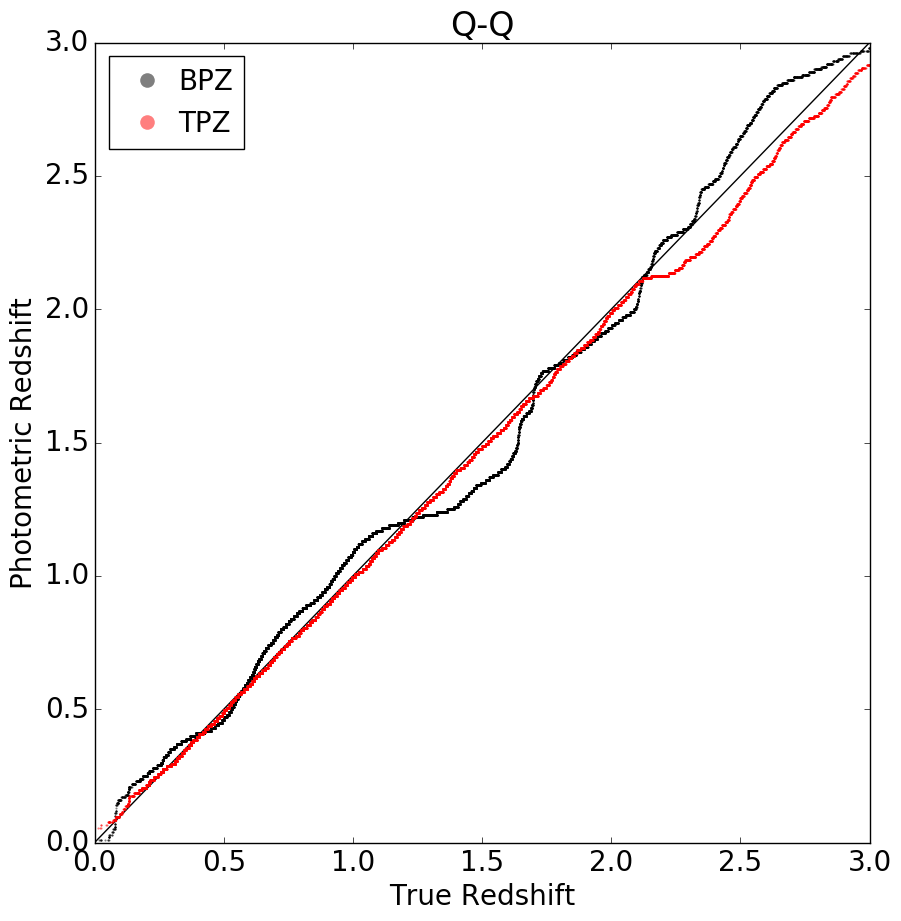
\includegraphics[width=10cm]{figures/qq_BPZ_TPZ.png}
\caption{Example of a Q-Q plot, using $z_\mathrm{true}$ and $z_\mathrm{phot}$, from the BPZ and TPZ estimators.}\label{fig:qq}
\end{center}
\end{figure*}


\subsection{Ideas for ``Real-World'' Science Tests}\label{ssec:more}

Instead of comparing the general performance of photo-$z$ estimators, we could compare them in specific real-world situations that represent some of the early science uses of Level 2 photo-$z$. Here is a short list of ideas.

\textbf{Cluster Identification:} take a line-of-sight from the simulated catalog with a known cluster, run the photometry through different algorithms, see which ones identify the cluster first/best.

\textbf{Supernova Classification:} Rahul is working on how including photo-$z$ helps SN classification, so perhaps we could see which algorithm produces the most useful photo-$z$ for likely SN hosts.

\textbf{Star/Galaxy Photometric Separation:} The Euclid catalog doesn't include $z=0$ stars, but we could insert some and see how well the different algorithms are at picking them out, either by including stellar templates to actively identify them, or by passively identifying stars by how they fail to return a decent photo-$z$.

\section{Conclusions}

For now, our interim recommendations are listed up front in the Introduction.

\bibliography{lsst,refs_ads}

\end{document}
